%  LaTeX support: latex@mdpi.com
%=================================================================
\documentclass[symmetry,article,submit,moreauthors]{Definitions/mdpi}

%=================================================================
% MDPI internal commands - do not modify
\firstpage{1}
\makeatletter
\setcounter{page}{\@firstpage}
\makeatother
\pubvolume{1}
\issuenum{1}
\articlenumber{0}
\pubyear{2026}
\copyrightyear{2026}
\datereceived{ }
\daterevised{ }
\dateaccepted{ }
\datepublished{ }

%=================================================================
\usepackage{amsmath,amssymb}
\usepackage{xcolor}
% highlighted-changes switch: \hltrue = changes shown in blue (version for the editor), \hlfalse = clean version
\newif\ifhl
\hlfalse
\newcommand{\TODO}[1]{{\color{red}\textbf{[TODO: #1]}}}
\newcommand{\rev}[1]{\ifhl{\color{blue}#1}\else#1\fi}
% generated by make_tex_r1.py -- do not edit
\makeatletter
\newcommand{\N}[1]{\@ifundefined{num@#1}{\textbf{[n/a: \detokenize{#1}]}}{\csname num@#1\endcsname}}
\makeatother
\expandafter\def\csname num@b1.cheb80.dt1e-4.l2\endcsname{\ensuremath{1.07\times10^{-5}}}
\expandafter\def\csname num@b1.cheb80.l2\endcsname{\ensuremath{5.37\times10^{-5}}}
\expandafter\def\csname num@b1.cheb80.time\endcsname{0.2}
\expandafter\def\csname num@b1.fh_K32.l2\endcsname{\ensuremath{(8.29\pm1.43)\times10^{-4}}}
\expandafter\def\csname num@b1.ratio.fh_K32_cheb80\endcsname{15}
\expandafter\def\csname num@b1.ratio.ode_fh_K32\endcsname{2.3}
\expandafter\def\csname num@b1.ratio.van_fhK32\endcsname{83}
\expandafter\def\csname num@b1.ratio.van_fhK32.ci\endcsname{[64, 104]}
\expandafter\def\csname num@b1.ratio.van_fhK32.linf\endcsname{51}
\expandafter\def\csname num@b1.ratio.van_fhK32.range\endcsname{63--117}
\expandafter\def\csname num@b1.speed.fh_K32_cheb80\endcsname{1213}
\expandafter\def\csname num@b1.speed.van_fhK32\endcsname{8.3}
\expandafter\def\csname num@b1.van.l2\endcsname{\ensuremath{(6.86\pm1.59)\times10^{-2}}}
\expandafter\def\csname num@b2.cheb80.l2\endcsname{\ensuremath{5.10\times10^{-5}}}
\expandafter\def\csname num@b3.cheb.l2\endcsname{\ensuremath{2.89\times10^{-5}}}
\expandafter\def\csname num@bal.dE_hard\endcsname{0.071}
\expandafter\def\csname num@bal.frac_hard\endcsname{0.018\%}
\expandafter\def\csname num@bal.id_err\endcsname{\ensuremath{4.4\times10^{-16}}}
\expandafter\def\csname num@bal.int_b_soft\endcsname{\ensuremath{4.11\times10^{-6}}}
\expandafter\def\csname num@bal.int_r_hard\endcsname{\ensuremath{1.28\times10^{-5}}}
\expandafter\def\csname num@en.max_diff\endcsname{\ensuremath{2.17\times10^{-6}}}
\expandafter\def\csname num@en.min_step\endcsname{\ensuremath{1.34\times10^{-3}}}
\expandafter\def\csname num@en.n_runs\endcsname{10}
\expandafter\def\csname num@en.nonzero\endcsname{1}
\expandafter\def\csname num@en.van_n\endcsname{4}
\expandafter\def\csname num@en.van_viol\endcsname{0}
\expandafter\def\csname num@ident.S001\endcsname{0.022}
\expandafter\def\csname num@ident.S005\endcsname{0.49}
\expandafter\def\csname num@ident.S01\endcsname{1.47}
\expandafter\def\csname num@ident.cl001\endcsname{53\%}
\expandafter\def\csname num@ident.cl005\endcsname{2.6\%}
\expandafter\def\csname num@ident.se001\endcsname{45\%}
\expandafter\def\csname num@inv.ratio_mean\endcsname{0.70}
\expandafter\def\csname num@inv.ratio_range\endcsname{0.61--0.73}
\expandafter\def\csname num@inv.steps\endcsname{18}
\expandafter\def\csname num@kk.cgl_soft_gain\endcsname{5}
\expandafter\def\csname num@kk.hard128.l2\endcsname{\ensuremath{(6.57\pm1.80)\times10^{-3}}}
\expandafter\def\csname num@kk.hard32.l2\endcsname{\ensuremath{(8.29\pm1.43)\times10^{-4}}}
\expandafter\def\csname num@kk.hard64.l2\endcsname{\ensuremath{(1.46\pm0.42)\times10^{-3}}}
\expandafter\def\csname num@kk.soft64.l2\endcsname{\ensuremath{(9.93\pm1.56)\times10^{-2}}}
\expandafter\def\csname num@kk.soft64.wall\endcsname{5.7}
\expandafter\def\csname num@mbp.excess\endcsname{\ensuremath{1.6\times10^{-2}}}
\expandafter\def\csname num@mbp.excess_all\endcsname{1.6\%}
\expandafter\def\csname num@mbp.max_b1\endcsname{1.0162}
\expandafter\def\csname num@mbp.max_hard\endcsname{1.0014}
\expandafter\def\csname num@mbp.max_van\endcsname{1.0084}
\expandafter\def\csname num@ode.compat.0.01.l2\endcsname{\ensuremath{1.89\times10^{-3}}}
\expandafter\def\csname num@ode.compat.0.1.l2\endcsname{\ensuremath{1.47\times10^{-1}}}
\expandafter\def\csname num@ode.orig.0.01.l2\endcsname{\ensuremath{1.30\times10^{-3}}}
\expandafter\def\csname num@ode.orig.0.1.l2\endcsname{\ensuremath{1.02\times10^{-1}}}
\expandafter\def\csname num@s2d.fmax\endcsname{\ensuremath{1.26\times10^{-31}}}
\expandafter\def\csname num@s2d.fmin\endcsname{\ensuremath{8.71\times10^{-32}}}
\expandafter\def\csname num@s2d.growth\endcsname{5.4}
\expandafter\def\csname num@s2d.growth_range\endcsname{4.4--6.8}
\expandafter\def\csname num@s2d.smax\endcsname{\ensuremath{3.74\times10^{-31}}}
\expandafter\def\csname num@s2d.smin\endcsname{\ensuremath{1.26\times10^{-31}}}


%=================================================================
% Full title of the paper (Capitalized)
\Title{A Chebyshev-Coefficient Physics-Informed Neural Network for the Allen--Cahn Equation: Exact Neumann Basis, A-Posteriori Energy Balance and Inverse Identification$^\dagger$}

% This paper is an extended version of a conference abstract (MDPI conference-paper policy)
\conference{Abdiramanov, Z.; Zhumazhanov, E.; Urnek, D. Investigation of Physics-Informed Neural Networks for Solving the Allen-Cahn Equation. In Proceedings of the 4th International Conference: Constructive Mathematical Analysis (ICCMA 2026), 1--2 July 2026}

% Author Orchid ID
\newcommand{\orcidauthorA}{0009-0004-9631-6284} % Zhuldyz Issa
\newcommand{\orcidauthorB}{0009-0002-5513-712X} % Adil Nauryzbay
\newcommand{\orcidauthorC}{0000-0003-3820-7253} % Zhanars Abdiramanov
\newcommand{\orcidauthorD}{0009-0008-5187-6105} % Yessimkhan Zhumazhanov
\newcommand{\orcidauthorE}{0009-0009-0099-4408} % Dastan Urnek

% Authors, for the paper (add full first names)
\Author{Zhuldyz Issa $^{1}$\orcidA{}, Adil Nauryzbay $^{1}$\orcidB{}, Zhanars Abdiramanov $^{1,2,}$*\orcidC{}, Yessimkhan Zhumazhanov $^{1}$\orcidD{} and Dastan Urnek $^{1}$\orcidE{}}

% MDPI internal command: Authors, for metadata in PDF
\AuthorNames{Zhuldyz Issa, Adil Nauryzbay, Zhanars Abdiramanov, Yessimkhan Zhumazhanov and Dastan Urnek}

% Affiliations / Addresses
\address{%
$^{1}$ \quad Department of Mathematics and Mathematical Modeling, Abai Kazakh National Pedagogical University, Almaty 050010, Kazakhstan\\
$^{2}$ \quad Institute of Information and Computational Technologies, Almaty 050010, Kazakhstan}

% Contact information of the corresponding author
\corres{Correspondence: zh.abdiramanov@abaiuniversity.edu.kz}

% Abstract (Do not insert blank lines, i.e. \\)
\abstract{Physics-informed neural networks (PINNs) are rarely compared with strong classical baselines or checked against the structure of the equation they solve. We study a PINN for the one-dimensional Allen--Cahn equation in which a network of time alone outputs the coefficients of a Chebyshev expansion that satisfies the Neumann condition exactly; spatial derivatives are exact, and a two-dimensional Fourier variant preserves reflection symmetry by construction. Against a certified reference solution and five seeds, the network is \N{b1.ratio.van_fhK32} times more accurate than a space--time PINN on a reaction-dominated benchmark, but classical Chebyshev collocation is a further \N{b1.ratio.fh_K32_cheb80} times more accurate and orders of magnitude faster; a diffusion-active benchmark and one with sharp interfaces are also reported. An energy penalty is inactive whenever the residual is small. Instead, we prove, and verify in Lean~4, an a-posteriori energy balance that bounds the energy growth of any trained trajectory by its PDE residual and boundary defect, and we measure both. Two effects reported in an earlier version, loss of accuracy at large mode numbers and a systematic bias in the recovered interface parameter, are shown to be artefacts of a weak boundary penalty and of the optimizer's starting value.
}

% Keywords
\keyword{physics-informed neural networks; Allen--Cahn equation; Chebyshev polynomials; Neumann boundary conditions; energy balance; maximum bound principle; inverse problems; symmetry; Lean 4}

\MSC{65M99; 35K57; 68T07}

%=================================================================

\begin{document}

\section{Introduction}

The Allen--Cahn equation~\cite{AllenCahn}
\begin{equation}\label{eq:AC-intro}
u_t = \varepsilon^2 \Delta u - f(u), \qquad f(u) = u^3-u = F'(u), \qquad F(u)=\tfrac14(u^2-1)^2,
\end{equation}
is a prototypical reaction--diffusion gradient flow describing phase separation in binary alloys, and it is the archetypal example used to develop and benchmark structure-preserving numerical schemes for the wider class of Ginzburg--Landau phase-field models~\cite{Du_review}. Two structural properties make Equation~\eqref{eq:AC-intro} a natural test bed for a journal devoted to symmetry. First, the double-well potential $F$ is invariant under the reflection $u\mapsto-u$, and this symmetry, together with the variational structure $u_t=-\delta E/\delta u$ of the Ginzburg--Landau free energy $E[u]=\int_\Omega(\frac{\varepsilon^2}{2}|\nabla u|^2+F(u))\,dx$, forces the continuous energy-dissipation law $dE/dt=-\|u_t\|^2_{L^2}\le0$ and the maximum bound principle $|u_0|\le1\Rightarrow|u(\cdot,t)|\le1$~\cite{ref_Du2021b}. Second, on domains with reflection or rotational symmetry, a symmetric initial condition produces a solution that remains symmetric for all time, because the isotropic Laplacian and the odd nonlinearity $f$ both commute with the corresponding symmetry group. Numerical methods that do not respect these properties can produce spurious energy growth, solutions outside $[-1,1]$, or artificially broken symmetry, which is why stability analysis in energy norms has been central to the design of discrete schemes for hyperbolic conservation laws~\cite{Baishemirov_Symmetry} and fractional flow models~\cite{Baigereyev_Math}, and why high-order structure-preserving spectral schemes remain an active research area for nonlocal and nonlinear diffusion problems~\cite{Shiyapov2026}.

Physics-informed neural networks (PINNs)~\cite{Raissi} approximate the solution of a PDE by a neural network trained to minimize the residual of the equation at a set of collocation points, together with initial- and boundary-condition losses. PINNs are mesh-free, extend naturally to irregular domains and high dimensions, and are compatible with data assimilation and inverse problems~\cite{Karniadakis2021,Yang_PINN,Lu_DeepXDE}, and their rapid growth has produced several recent surveys~\cite{Khanra2026,Pateras2023}; operator-learning variants such as DeepONet~\cite{Lu_DeepONet,Li_DeepONetExt2025} and the Fourier Neural Operator~\cite{Li_FNO} extend the idea to families of problems. For the Allen--Cahn equation specifically, however, vanilla PINNs face two well-documented difficulties. First, for small $\varepsilon$ the solution develops a sharp interface of width $O(\varepsilon)$, and the spectral bias of fully connected networks toward low frequencies makes this interface hard to resolve~\cite{Wight,ref_Rahaman2019}, a phenomenon that a neural-tangent-kernel analysis traces to the network's training dynamics rather than its expressive power alone~\cite{Wang_NTK2022}; adaptive sampling~\cite{Wight}, causal training~\cite{Wang_causal}, sequential/backward-compatible training~\cite{Mattey}, and spatially adaptive Fourier-feature encodings~\cite{Liu_FourierBias2025} have all been proposed to mitigate this. More generally, the training of PINNs is hampered by loss-term imbalance and by the ill-conditioning of the differential operators in the residual~\cite{ref_Wang2021a,ref_Krishnapriyan2021,ref_Rathore2024}. Second, the standard PINN loss enforces only the pointwise PDE residual and provides no structural guarantee that the discrete energy decreases, even though this is the single most important qualitative property of the continuous solution.

\rev{Several recent works place a discretization inside the network, or add structure to the loss, and are the closest relatives of the present study. Networks whose only input is time and whose output is the vector of coefficients of a fixed spectral basis, with spatial derivatives taken exactly from the basis, were introduced by Xia, B\"ottcher and Chou~\cite{ref_Xia2023}, who treat linear transport, heat and Schr\"odinger equations on bounded (Chebyshev) and unbounded (Laguerre, Hermite) domains and also estimate a diffusivity from noisy data; related coefficient-space networks are neural spectral methods for parametric PDEs~\cite{ref_Du2024} and the neuro-spectral architectures of Bizzi et al.~\cite{ref_Bizzi2025}, in which the dynamics are learned in Fourier space and boundary conditions hold by the choice of basis. Neural Galerkin schemes~\cite{ref_Bruna2024} and evolutional networks~\cite{ref_Du2021a} march network parameters in time instead. For the Allen--Cahn equation, K\"ut\"uk and Yücel~\cite{ref_Kutuk2025} add a one-sided penalty on the time derivative of the energy to a coordinate-based PINN, an energy-based sequential training strategy was proposed in~\cite{Guo_EnergySeq2024}, energy dissipation is guaranteed by construction in networks built on the scalar auxiliary variable approach~\cite{ref_Zhang2024,ref_Lin2025}, and the maximum bound is enforced by a limiter in a learned fully discrete solver~\cite{ref_Geng2025}. Exactly imposing boundary conditions, periodicity or conservation laws through the architecture is also well established~\cite{ref_Dong2021,ref_Sukumar2022,ref_Lu2021,ref_CardosoBihlo2025}. Finally, for forward problems the established outcome is that classical solvers are faster and at least as accurate as PINNs, including for the one-dimensional Allen--Cahn equation~\cite{ref_Grossmann2024,ref_McGreivy2024}.}

A separate line of work builds symmetry directly into the PINN loss, training data, or architecture, rather than treating it as an emergent property of training. Symmetry-enhanced PINNs augment the loss with invariant-surface conditions derived from a PDE's Lie point symmetries~\cite{Zhang_SPINN2023,Zhang_SymGroup2023}; Lie-symmetry data augmentation generates additional, physically consistent training points from known symmetries~\cite{Brandstetter2022}; invariant PINNs restrict the network to be equivariant under a prescribed symmetry group for ordinary differential equations~\cite{Arora2024}; and symmetry-group-based domain decomposition uses a PDE's symmetry group to split the training domain into physically equivalent pieces~\cite{Liu_SymDD2024}. Closest in spirit to the present work, symmetry-preserving PINNs (S-PINNs) were introduced for nonlinear dynamical lattices to penalize violations of conserved quantities and symmetries that vanilla PINNs otherwise exhibit~\cite{Zhu_SPINN2022}. All of these approaches enforce symmetry through the loss function, through training data, or through equivariant layers; the Fourier-Spectral-PINN of Section~\ref{sec:2d} differs by enforcing reflection symmetry directly through the choice of \emph{basis functions} in the output representation, so that no loss term is responsible for it. This is a special case of the hard-constraint design cited above, and we claim only its demonstration for the two-dimensional Allen--Cahn equation.

On the numerical-analysis side, the scalar auxiliary variable (SAV) approach~\cite{Shen_SAV}, building on convex splitting~\cite{Eyre}, and its generalized~\cite{Huang_GSAV} and relaxed~\cite{Jiang_RSAV} variants, provide classical schemes with \emph{unconditional} energy stability at the cost of solving a linear system at every time step. A parallel and extensively studied family of structure-preserving schemes instead targets the discrete \emph{maximum principle} $\|u^n\|_\infty\le1$ alongside energy stability, via stabilized semi-implicit and exponential time differencing schemes~\cite{ref_Tang2016,Zhang_ETD2024}, high-order parametric integrating factor Runge--Kutta schemes~\cite{Gao_pIFRK2023}, maximum-principle-preserving discontinuous Galerkin methods~\cite{Du_MPPDG2022}, and linear finite-difference schemes in two and three dimensions~\cite{Feng_MPPFD2021,Kim_MPP3D2025}. Energy decay alone does not imply that such a bound holds, which is why admissibility ($|u|\le1$) has to be checked separately from energy monotonicity; we do so for every trained network below. High-order spectral collocation combined with a Fast Memory Algorithm has recently been used to obtain structure-preserving, high-accuracy solutions of nonlocal nonlinear diffusion equations closely related to Allen--Cahn~\cite{Shiyapov2026}.

\textbf{Scope and contributions.} \rev{We do not claim that coefficient-space networks or energy penalties are new; both are cited above. This article is a careful and reproducible evaluation of a Chebyshev-coefficient PINN for the Allen--Cahn equation against strong baselines, and its contributions are the following. (i)~An exactly Neumann-compatible Chebyshev basis for the coefficient network (Section~\ref{sec:spectral}), together with the observation that the commonly used soft boundary penalty, when rescaled with the mode number, produces a spurious loss of accuracy at large $K$ (Section~\ref{sec:results-k}). (ii)~A forward-problem study on three benchmarks of increasing difficulty (a reaction-dominated one, a diffusion-active one, and a one with sharp interfaces), five seeds per configuration, a certified high-accuracy reference solution and the classical Chebyshev collocation solver as the strong baseline, with maximum-bound and energy-monotonicity diagnostics for every trained network (Section~\ref{sec:results-forward}). (iii)~An a-posteriori energy balance, valid for \emph{any} trained trajectory and machine-checked in Lean~4, which bounds the energy growth of the learned solution by its PDE residual and boundary defect; the residual and the defect are measured for every trained network (Sections~\ref{sec:balance} and~\ref{sec:results-balance}, Appendix~\ref{app:perturbed}). (iv)~A controlled ablation of the energy penalty (weight, regime), which shows that the penalty is inactive whenever the residual is small (Section~\ref{sec:results-energy}). (v)~A diagnosis of why the joint training of the network and of $\varepsilon$ returns an estimate that depends on the starting value, an estimator that does not have this defect, and a comparison with a classical least-squares estimator including the question of identifiability (Section~\ref{sec:results-inverse}). (vi)~The demonstration that restricting the Fourier basis preserves reflection symmetry of the two-dimensional solution to round-off (Section~\ref{sec:2d-results}). The method is not offered as a replacement for classical solvers on the forward problem, and Section~\ref{sec:niche} states what we think its legitimate niche is.}

This article is an extended version of a conference abstract~\cite{ICCMA2026abstract} that outlined the Spectral-PINN and energy-constrained-loss idea; the present manuscript adds the full formulation, the two-dimensional symmetric extension, the multi-seed experiments, the energy balance and the Lean~4 formalization of Appendix~\ref{app:lean}, none of which appeared in the original abstract.
%%%%%%%%%%%%%%%%%%%%%%%%%%%%%%%%%%%%%%%%%%
\section{Materials and Methods}

\subsection{Problem Formulation, Energy Dissipation and Benchmarks}\label{sec:problem}

Let $\Omega=[-1,1]$ and $t\in[0,T]$. We consider
\begin{equation}\label{eq:AC}
u_t = \varepsilon^2 u_{xx} - f(u), \qquad u_x(\pm1,t)=0, \qquad u(x,0)=u_0(x),
\end{equation}
with $f(u)=u^3-u$. The Ginzburg--Landau free energy is $E[u]=\int_{-1}^{1}\bigl(\frac{\varepsilon^2}{2}u_x^2+F(u)\bigr)\,dx$.

\rev{\emph{Initial condition.} The initial condition must satisfy the compatibility condition $u_0'(\pm1)=0$, otherwise the solution has an initial boundary layer and the problem is not well posed at $t=0$ in the classical sense. The condition $u_0(x)=x^2\cos(\pi x)$ that is widely used for the Allen--Cahn PINN benchmark with \emph{periodic} boundary conditions~\cite{Raissi,ref_Kutuk2025} does not satisfy it for the Neumann problem ($u_0'(-1)=2$, $u_0'(1)=-2$), and it was used with Neumann conditions in the first version of this study. All experiments reported here use the Neumann-compatible condition
\begin{equation}\label{eq:IC}
u_0(x)=\tfrac12\bigl(\cos(\pi x)-\cos^2(\pi x)\bigr)=\sin^2\!\bigl(\tfrac{\pi x}{2}\bigr)\cos(\pi x),
\end{equation}
which has the same values at $x=0,\pm\tfrac12,\pm1$ as $x^2\cos(\pi x)$ (namely $0,0,-1$), $|u_0|\le\tfrac18$ in the interior, and $u_0'(\pm1)=0$. Appendix~\ref{app:orig} repeats the principal forward experiments with the original condition and shows that none of the conclusions depends on this choice.}

\rev{\emph{Benchmarks.} Three benchmarks are used, because the original choice ($\varepsilon=0.01$, $T=1$) turned out to test the PDE only weakly. B1 is $\varepsilon=0.01$, $T=1$ (the original). Its solution is dominated by the reaction term: no interface forms before $t\approx3$, and neglecting diffusion altogether (the closed-form solution of $u'=u-u^3$ at every $x$) already gives an $L^2$ error of \N{ode.compat.0.01.l2} at $t=1$ (Table~\ref{tab:forward}). B2 is $\varepsilon=0.1$, $T=1$: the solution is smooth but diffusion matters (the reaction-only error is \N{ode.compat.0.1.l2}), so a method that solves the PDE must beat that number clearly. B3 is $\varepsilon=0.05$, $T=5$: sharp interfaces ($\max|u_x|\approx14$) form around $t=3$--$5$, and a polynomial of degree $K=32$ cannot represent the solution at $T=5$ to better than $L^2\approx10^{-2}$ while $K=64$ can ($2\times10^{-4}$), so B3 probes whether the network can learn interface dynamics.}

\begin{Theorem}[Continuous energy dissipation]\label{thm:energy}
Any smooth solution of Equation~\eqref{eq:AC} satisfies $\dfrac{dE}{dt}=-\displaystyle\int_{-1}^{1}u_t^2\,dx\le0$.
\end{Theorem}
\begin{proof}
Differentiating $E$ under the integral sign and integrating $\int u_x u_{xt}\,dx$ by parts (the boundary term vanishes by the Neumann condition) gives $dE/dt=\int(-\varepsilon^2u_{xx}+f(u))u_t\,dx=-\int u_t^2\,dx$, using Equation~\eqref{eq:AC}.
\end{proof}

This theorem is the structural target that the energy-constrained loss (Section~\ref{sec:energy-loss}) attempts to enforce approximately at the level of the trained network. \rev{Section~\ref{sec:balance} gives its counterpart for a network that does \emph{not} solve the PDE exactly.}

\subsection{Reference Solution and Baseline Methods}\label{sec:cheb-baseline}

\rev{\emph{Reference solution.} All errors are measured against a spectral reference: Chebyshev collocation on the Gauss--Lobatto nodes with the two Neumann rows used to eliminate the wall unknowns, and the stiff integrator Radau (rtol $10^{-11}$) in time. It was certified by $N$-doubling, tolerance tightening, a second integrator and an independent ghost-node finite-difference solution, with agreement to $\le10^{-8}$ for all cases used here (Appendix~\ref{app:ref}). Predictions and reference are compared on the same 200 equispaced points of $[-1,1]$, with $\|e\|_{L^2}=(\sum_ie_i^2\,\delta x)^{1/2}$, $\delta x=2/199$, and $\|e\|_{L^\infty}=\max_i|e_i|$. The first version used a first-order finite-difference reference whose wall rows were inconsistent with the Neumann condition; its error (up to $4\times10^{-3}$ near the walls at early times) was small compared with the PINN errors but not compared with the classical baseline.}

\emph{Classical baseline.} As a classical point of comparison, playing the role of the spectral scheme of~\cite{Shiyapov2026} for the (local) Allen--Cahn equation, we discretize Equation~\eqref{eq:AC} on the Chebyshev--Gauss--Lobatto nodes $x_j=\cos(j\pi/N)$ using the differentiation matrix $D$ of~\cite{Trefethen}, with a first-order semi-implicit (IMEX) time step: the diffusion term is implicit and the reaction term $f(u^n)$ is explicit. Homogeneous Neumann conditions are imposed by boundary bordering. \rev{We use $N=80$ and $\delta t=5\times10^{-4}$; the error of this scheme is dominated by the first-order time stepping and falls proportionally to $\delta t$ (Table~\ref{tab:forward}). The scheme is used only as an accuracy and cost reference; it is not claimed to reproduce the Fast Memory Algorithm of~\cite{Shiyapov2026}.}

\emph{Vanilla PINN.} The second baseline is a vanilla space--time PINN, which represents $u(x,t)\approx\mathcal N(x,t;\theta)$ by a fully connected network with $\tanh$ activations (three hidden layers of width 64), trained by minimizing $\mathcal L=\mathcal L_{\rm PDE}+\lambda_{\rm IC}\mathcal L_{\rm IC}+\lambda_{\rm BC}\mathcal L_{\rm BC}$ with $\lambda_{\rm IC}=\lambda_{\rm BC}=10$, where $\mathcal L_{\rm PDE}$ is the mean-squared residual of Equation~\eqref{eq:AC} on a $80\times80$ grid of collocation points (all derivatives via automatic differentiation), $\mathcal L_{\rm IC}$ fits $u_0$, and $\mathcal L_{\rm BC}$ penalizes $|\mathcal N_x(\pm1,t)|^2$. Adam with cosine-annealed learning rate $10^{-3}$, 8000 epochs. This is the formulation used throughout the Allen--Cahn PINN literature~\cite{Raissi,Wight,Mattey}.

\subsection{Coefficient-Space PINN (Spectral-PINN)}\label{sec:spectral}

If $u(x)=\sum_{k=0}^{K}c_kT_k(x)$ is a truncated Chebyshev series, its derivative is again a Chebyshev series $u'(x)=\sum_{k=0}^{K-1}b_kT_k(x)$ whose coefficients are obtained from $\{c_k\}$ by the closed-form backward recurrence
\begin{equation}\label{eq:cheb-recurrence}
b_K=0,\qquad b_{k-1}=b_{k+1}+2kc_k\ \ (k=K,\dots,1),\qquad b_0\leftarrow b_0/2.
\end{equation}
Because Equation~\eqref{eq:cheb-recurrence} is linear in $\{c_k\}$, it defines a fixed $(K+1)\times(K+1)$ matrix $D_c$ with $\mathbf{b}=D_c\mathbf{c}$; the second derivative uses $D_c^2$. We verified $D_c$ against analytic derivatives of a smooth test function (errors $10^{-11}$--$10^{-13}$ for $K=20$).\label{sec:cheb-coeff}

Following the idea of time-only coefficient networks~\cite{ref_Xia2023}, we replace the direct field parameterization $\mathcal N(x,t;\theta)\to u$ by a \emph{coefficient} parameterization
\begin{equation}\label{eq:spectral-pinn}
\mathbf c(t)=\mathcal N(t;\theta)\in\mathbb R^{K+1}, \qquad u(x,t)=\sum_{k=0}^{K}c_k(t)\,T_k(x),
\end{equation}
i.e., the network is a function of time alone (two hidden layers of width 64, $\tanh$) and outputs the instantaneous Chebyshev spectrum of the solution. Spatial derivatives entering the residual are computed exactly with $D_c,D_c^2$; the only derivative computed by automatic differentiation is $\dot{\mathbf c}(t)$, obtained by backpropagating through the network once per coefficient. The loss is
\begin{equation}\label{eq:loss}
\mathcal L=\mathcal L_{\rm PDE}+\lambda_{\rm IC}\,|\mathbf c(0)-\mathbf c_0|^2+\lambda_{\rm BC}\mathcal L_{\rm BC}+\lambda_E\mathcal L_E,\qquad
\mathcal L_{\rm PDE}=\Big\langle\tfrac12\|r(\cdot,t)\|_{L^2}^2\Big\rangle_t,
\end{equation}
with $r=u_t-\varepsilon^2u_{xx}+f(u)$, $\lambda_{\rm IC}=10$, $\lambda_{\rm BC}=1$ and $\mathbf c_0$ the Chebyshev projection of $u_0$. The time average is over $100\,T$ equispaced collocation times in $[10^{-4},T]$; before the PDE loss is switched on the network is pretrained for 1000 epochs to output the constant-in-time coefficient vector $\mathbf c_0$. Training uses Adam (learning rate $10^{-3}$, cosine annealing) for $6000+1500(T-1)$ epochs. The pointwise nonlinearity $f(u)$ has no closed-form action on the coefficients and is evaluated on a spatial grid; \rev{two spatial grids are used. \emph{As submitted:} 300 equispaced points with a plain mean over the grid. \emph{Revised:} $N=\max(300,4K+8)$ Gauss--Lobatto points with Clenshaw--Curtis weights, which makes the discrete $\|r\|_{L^2}^2$ and the discrete energy accurate quadratures and keeps the least-squares fit of $\mathbf c_0$ well conditioned (the Vandermonde matrix on 300 equispaced points has condition number $10^{10}$ at $K=128$ and $10^{15}$ for $K\ge192$).}

\rev{\emph{Neumann condition.} Two ways of imposing $u_x(\pm1,t)=0$ are compared. In the \emph{soft} variant of the first version, $\mathcal L_{\rm BC}$ penalizes $u_x(\pm1,t)=\sum_kc_k\,T_k'(\pm1)$ with $T_k'(1)=k^2$, $T_k'(-1)=(-1)^{k+1}k^2$, after dividing these vectors by $K^2$ to keep the entries $O(1)$; because the loss squares the residual, the effective weight of $u_x(\pm1)^2$ is $\lambda_{\rm BC}K^{-4}$, which is $10^{-6}$ at $K=32$ and $6\times10^{-8}$ at $K=64$. In the \emph{hard} (revised) variant the network does not output $\mathbf c$ but $K-1$ free numbers $\mathbf b$, and $\mathbf c=M\mathbf b$ with
\begin{equation}\label{eq:neumann-basis}
\varphi_k=T_k-\frac{k^2}{(k+2)^2}\,T_{k+2},\qquad k=0,\dots,K-2 .
\end{equation}
Since $T_k'(1)=k^2$ and $T_k'(-1)=(-1)^{k+1}k^2$, one has $\varphi_k'(\pm1)=0$ for all $k$; the $K-1$ polynomials $\varphi_k$ are linearly independent (distinct degrees $k+2$ for $k\ge1$ and $\varphi_0=1$, $\varphi_1=T_1-\frac19T_3$), and the polynomials of degree $\le K$ with $p'(\pm1)=0$ form a space of dimension $K-1$ (two independent linear conditions on $\mathbb P_K$), so they span it. The Neumann condition then holds identically, $\mathcal L_{\rm BC}\equiv0$, and the boundary term of the energy balance in Section~\ref{sec:balance} vanishes.}

\subsection{Energy-Constrained Training}\label{sec:energy-loss}

To translate Theorem~\ref{thm:energy} into a training signal, we evaluate the discrete Ginzburg--Landau energy $E_\theta(t)$ (on the spatial grid above, with the exact spectral derivative for $u_x$) at $M+1$ time checkpoints $0=\tau_0<\dots<\tau_M=T$, with $M=10\,T$ (that is, spacing $0.1$), and add the one-sided penalty
\begin{equation}\label{eq:Lenergy}
\mathcal L_E(\theta)=\sum_{i=0}^{M-1}\big[\max\big(0,\,E_\theta(\tau_{i+1})-E_\theta(\tau_i)\big)\big]^2
\end{equation}
to the loss, with weight \rev{$\lambda_E=50$ unless stated otherwise (the value used in all runs of the first version; Section~\ref{sec:results-energy} varies it from $1$ to $5000$)}. Equation~\eqref{eq:Lenergy} is zero whenever the network's own energy trajectory is already monotonically decreasing at the checkpoints; it is a soft, trainable analogue of the algebraic energy identity that SAV-type schemes~\cite{Shen_SAV} enforce exactly. \rev{Penalizing energy growth in a PINN loss for Allen--Cahn was proposed in~\cite{ref_Kutuk2025}, with $\partial E/\partial t$ obtained by automatic differentiation at collocation points; our variant penalizes finite increments of the checkpointed energy of a coefficient network, with an exact spectral $u_x$. Energy-based sampling strategies for gradient-flow PINNs are discussed in~\cite{Guo_EnergySeq2024}.} \rev{For evaluation, ``energy violations'' are counted as the number of consecutive pairs of an equispaced time grid at which the energy increases by more than $10^{-10}$; the energy is computed by Clenshaw--Curtis quadrature on $4K+8$ nodes, which is exact for the polynomial integrand, and the count is reported for grids with spacing $0.02$, $0.002$ and $2\times10^{-4}$, i.e.\ much finer than the penalty checkpoints.}

\subsection{A-Posteriori Energy Balance for a Trained Trajectory}\label{sec:balance}

\rev{Theorem~\ref{thm:energy} holds for exact solutions. A trained network satisfies the PDE only up to the residual $r=u_t-\varepsilon^2u_{xx}+f(u)$ and, in the soft variant, the Neumann condition only up to a defect. For $u(x,t)=\sum_kc_k(t)T_k(x)$ with $c\in C^1$ the following identity holds for every $t$, by two integrations by parts in $x$ (Appendix~\ref{app:perturbed}, Proposition~\ref{prop:pde-identity}):
\begin{equation}\label{eq:balance-main}
\frac{dE}{dt}=-\|u_t\|^2+\langle r,u_t\rangle+\varepsilon^2\bigl[u_xu_t\bigr]_{x=-1}^{x=1}\ \le\ \tfrac12\|r\|^2-\tfrac12\|u_t\|^2+\varepsilon^2\bigl[u_xu_t\bigr]_{x=-1}^{x=1},
\end{equation}
where $\|\cdot\|$ and $\langle\cdot,\cdot\rangle$ are those of $L^2(-1,1)$. Consequently, for $0\le s\le t\le T$,
\begin{equation}\label{eq:balance-int}
E(t)+\tfrac12\int_s^t\|u_t\|^2\,d\tau\ \le\ E(s)+\tfrac12\int_s^t\|r\|^2\,d\tau+\int_s^t\beta\,d\tau,\qquad\beta=\varepsilon^2[u_xu_t]_{-1}^{1}.
\end{equation}
With the hard Neumann basis $\beta\equiv0$. Equation~\eqref{eq:balance-int} does not say that a trained network dissipates energy; it says that the energy of the learned solution can grow only through the residual and the boundary defect, both of which are computable a posteriori to round-off, because $r^2$ and the energy integrand are polynomials in $x$ and are integrated exactly by Clenshaw--Curtis quadrature. We evaluate them for every trained network (Section~\ref{sec:results-balance}). The identity and the inequalities are machine-checked in Lean~4 (Appendix~\ref{app:perturbed}); that this is the right link between the formalized gradient-flow theorem and the trained network was the point of a reviewer's remark on the first version.}

\subsection{Inverse Problem: Recovering the Interface Parameter}\label{sec:inverse}

For the inverse problem $\varepsilon$ is unknown and synthetic observations $u_{\rm obs}$ of the reference solution (with a known $\varepsilon_{\rm true}$), sampled at $n_x=40$ equispaced points and at the five times $t\in\{0.2,0.4,0.6,0.8,1.0\}$ and optionally corrupted by Gaussian noise of absolute standard deviation $\sigma$, are given. The loss is $\mathcal L=\lambda_{\rm PDE}\mathcal L_{\rm PDE}(\varepsilon)+\lambda_{\rm IC}\mathcal L_{\rm IC}+\lambda_{\rm BC}\mathcal L_{\rm BC}+\lambda_{\rm data}\mathcal L_{\rm data}$ with $\mathcal L_{\rm data}=\langle(u_\theta(x_{\rm obs},t_{\rm obs})-u_{\rm obs})^2\rangle$ and $(\lambda_{\rm PDE},\lambda_{\rm IC},\lambda_{\rm BC},\lambda_{\rm data})=(50,10,1,2)$ unless stated otherwise. Three estimators are compared. \emph{Joint Adam} (the procedure of the first version): $\log\varepsilon$ is an additional trainable scalar updated by Adam with a learning rate $10\times$ that of the network, starting from $\varepsilon_{\rm init}$. \rev{\emph{Variable projection:} the residual is linear in $\varepsilon^2$, so for the current network the minimizer of $\mathcal L_{\rm PDE}$ over $\varepsilon^2$ is the closed-form least-squares value $\varepsilon^2_{\rm LS}=\langle u_t+f(u),u_{xx}\rangle/\langle u_{xx},u_{xx}\rangle$; this value, relaxed with weight $0.1$, replaces the trainable scalar, after a data-fitting phase of 3000 epochs in which the PDE loss is off. \emph{Classical least squares:} nonlinear least squares for $\log\varepsilon$ with the Chebyshev collocation solver as forward model, started from the same $\varepsilon_{\rm init}$ (an exact-data ``inverse crime'' in the noise-free case, which is why the noisy runs, with an independently computed reference, are the meaningful comparison).}

\subsection{Two-Dimensional Symmetric Extension}\label{sec:2d}

To test symmetry preservation directly, we consider the periodic domain $[-\pi,\pi]^2$ with the reflection-symmetric initial condition $u_0(x,y)=0.4\cos(2x)\cos(2y)$, invariant under $x\mapsto-x$, $y\mapsto-y$, and $x\leftrightarrow y$. Since the isotropic Laplacian and $f$ commute with these reflections, the exact solution remains symmetric for all $t$. The Fourier-Spectral-PINN represents $u(x,y,t)=\sum_{m,n=0}^{M}c_{mn}(t)\cos(mx)\cos(ny)$; because every basis function is even in $x$ and in $y$, $u(-x,y,t)=u(x,y,t)$ and $u(x,-y,t)=u(x,y,t)$ hold \emph{by construction}, independent of training quality, and the Laplacian is diagonal in mode space, $\Delta[\cos(mx)\cos(ny)]=-(m^2+n^2)\cos(mx)\cos(ny)$. As a control, the vanilla PINN is given the periodic (but not reflection-symmetric) input encoding $(\cos x,\sin x,\cos y,\sin y,t)$, so both methods handle periodicity exactly and only the reflection symmetry is architecture-dependent. We report the violation metric $S(t)=\langle(u(x,y,t)-u(-x,y,t))^2\rangle+\langle(u(x,y,t)-u(x,-y,t))^2\rangle$ for both methods, evaluated on $x_i=-\pi+ih$, $h=2\pi/(n-1)$, so that the reflection maps grid points to grid points (Appendix~\ref{app:sym}). This experiment is unchanged from the first version; it does not involve a Neumann condition.

\subsection{Implementation and Evaluation Protocol}\label{sec:protocol}

\rev{All networks are multilayer perceptrons with $\tanh$ activations in double precision, trained with Adam on one CPU thread of an Intel Core i5-9400F (six cores); runs of a group were executed concurrently, so wall-clock times are comparable inside a table but are not a clean benchmark (a separate timing measurement is reported in Table~\ref{tab:forward}). Seeds are $\{42,123,7,2024,99\}$ unless stated otherwise; ``mean $\pm$ SD'' uses the sample standard deviation ($n-1$). The statistic behind every ratio of errors is the ratio of the seed means, and confidence intervals are 95\% percentile bootstrap intervals (20\,000 resamples of the seeds, independently for numerator and denominator). The maximum-bound diagnostic is $\max_{x,t}|u|$ on a $1001\times(100T+1)$ grid. Source code, the certified reference and all raw results are provided with the submission and in the repository cited in the Data Availability Statement.}

\subsection{Formal Verification}\label{sec:lean}

Numerical stability proofs for gradient-flow schemes typically hinge on a small number of algebraic manipulations---polarization identities, and the step in a discrete Gr\"onwall argument where a squared-norm term is moved from the right- to the left-hand side of an inequality before dividing. A review of an earlier, unrelated Allen--Cahn manuscript from this research group identified exactly this class of error: a term was silently dropped when both sides of an inequality were multiplied through in the course of a discrete-Gr\"onwall stability proof. Interactive theorem provers such as Lean~\cite{DeMouraUllrich2021} eliminate this class of error by construction, and have recently been used to formalize physical theories~\cite{Bobbin2023,Ugwuanyi2025} and numerical algorithms~\cite{Tsachouridis2020}; mechanized proofs of numerical-analysis statements also exist in Coq and Isabelle~\cite{ref_Boldo2013,ref_Tekriwal2021}. We formalized and machine-checked, in Lean~4 with Mathlib, (i) the polarization identity $2a(a-b)=a^2-b^2+(a-b)^2$ and a discrete Gr\"onwall step (Appendix~\ref{app:lean}), (ii) Theorem~\ref{thm:energy} in its abstract form: for any gradient flow $c'=-\nabla E(c)$ on a real Hilbert space, $\frac{d}{dt}E(c)=-\|c'\|^2$ (Theorem~\ref{thm:app-gradflow}), and \rev{(iii) its extension to arbitrary differentiable trajectories, i.e., the energy balance of Section~\ref{sec:balance} with residual and defect, together with the integrated and discrete-time bounds and the integration by parts for polynomials (Appendix~\ref{app:perturbed}). The scope of these statements is exactly what they say: (ii) concerns exact gradient flows and says nothing about a trained network; (iii) is conditional on the residual and the boundary defect, which are measured, not assumed.} All theorems compile against Lean~4.33.1 and Mathlib without \texttt{sorry} and depend only on the axioms \texttt{propext}, \texttt{Classical.choice} and \texttt{Quot.sound}.
%%%%%%%%%%%%%%%%%%%%%%%%%%%%%%%%%%%%%%%%%%
\section{Results}

\subsection{Forward Problem}\label{sec:results-forward}

\rev{Table~\ref{tab:forward} compares the methods on the three benchmarks of Section~\ref{sec:problem}. The Spectral-PINN rows are given in two versions: ``as submitted'' (soft Neumann penalty, 300 equispaced collocation points) and ``revised'' (hard Neumann basis, Gauss--Lobatto collocation). Errors are measured at $t=1$ ($t=5$ for B3) against the certified reference on the common 200-point grid; ``mean $\pm$ SD'' is over $n$ seeds. The last two columns give the maximum of $|u|$ over $x$ and $t$ (maximum bound principle) and the number of energy increases among the consecutive pairs of a grid of spacing $0.02$ (Section~\ref{sec:energy-loss}).}

\begin{table}[H]
\caption{\rev{Forward problem on the three benchmarks. Errors against the certified reference on the common 200-point grid, mean $\pm$ SD over $n$ seeds; ``Energy incr.'' = number of increases of the energy over the intervals of a grid of spacing $0.02$ (total over seeds, $50T$ intervals per run); $\max|u|$ is the largest value over all runs of the row. Time is the training time of one run on an idle single core (rows with $^\dagger$: mean over the main runs, which were executed concurrently and are not a clean timing); the classical time is the median of three solves. The vanilla PINN has 8000 Adam epochs, the Spectral-PINN 6000 (+1000 warm-up) for $T=1$.}\label{tab:forward}}
\footnotesize
\begin{tabularx}{\textwidth}{Xccccccc}
\toprule
\textbf{Method} & \textbf{Params} & $L^2$ error & $L^\infty$ error & $n$ & Time (s) & $\max|u|$ & Energy incr.\\
\midrule
\multicolumn{8}{l}{\textit{B1: $\varepsilon=0.01$, $T=1$ (error at $t=1$)}}\\
Chebyshev collocation, $N=80$, $\delta t=0.0005$ & 81 & \ensuremath{5.37\times10^{-5}} & \ensuremath{6.48\times10^{-5}} & 1 & 0.21 & -- & --\\
Chebyshev collocation, $N=80$, $\delta t=0.0001$ & 81 & \ensuremath{1.07\times10^{-5}} & \ensuremath{1.30\times10^{-5}} & 1 & 1.29 & -- & --\\
Reaction-only ODE ($\varepsilon=0$) & 0 & \ensuremath{1.89\times10^{-3}} & \textbf{--} & 1 & -- & -- & --\\
Vanilla PINN & 8577 & \ensuremath{(6.86\pm1.59)\times10^{-2}} & \ensuremath{(9.80\pm2.18)\times10^{-2}} & 4 & 2081$^\dagger$ & 1.0084 & 0/200\\
Vanilla PINN + L-BFGS & 8577 & \textbf{--} & \textbf{--} & \textbf{--} & \textbf{--} & \textbf{--} & \textbf{--}\\
Spectral-PINN, as submitted, $K=32$ & 6433 & \textbf{--} & \textbf{--} & \textbf{--} & \textbf{--} & \textbf{--} & \textbf{--}\\
\quad + energy penalty ($\lambda_E=50$) & 6433 & \textbf{--} & \textbf{--} & \textbf{--} & \textbf{--} & \textbf{--} & \textbf{--}\\
Spectral-PINN, as submitted, $K=64$ & 8513 & \ensuremath{(9.93\pm1.56)\times10^{-2}} & \ensuremath{(1.71\pm0.30)\times10^{-1}} & 4 & 410$^\dagger$ & 1.0162 & 0/200\\
Spectral-PINN, revised, $K=32$ & 6303 & \ensuremath{(8.29\pm1.43)\times10^{-4}} & \ensuremath{(1.92\pm0.36)\times10^{-3}} & 5 & 251$^\dagger$ & 1.0013 & 0/250\\
\quad + energy penalty ($\lambda_E=50$) & 6303 & \ensuremath{(8.29\pm1.45)\times10^{-4}} & \ensuremath{(1.92\pm0.36)\times10^{-3}} & 5 & 214$^\dagger$ & 1.0013 & 0/250\\
\quad + L-BFGS & 6303 & \textbf{--} & \textbf{--} & \textbf{--} & \textbf{--} & \textbf{--} & \textbf{--}\\
Spectral-PINN, revised, $K=64$ & 8383 & \ensuremath{(1.46\pm0.42)\times10^{-3}} & \ensuremath{(3.66\pm0.92)\times10^{-3}} & 5 & 587$^\dagger$ & 1.0014 & 0/250\\
Spectral-PINN, revised, $K=128$ & 12543 & \ensuremath{(6.57\pm1.80)\times10^{-3}} & \ensuremath{(1.24\pm0.01)\times10^{-2}} & 2 & 732$^\dagger$ & 1.0014 & 0/100\\
\midrule
\multicolumn{8}{l}{\textit{B2: $\varepsilon=0.1$, $T=1$}}\\
Chebyshev collocation, $N=80$, $\delta t=0.0005$ & 81 & \ensuremath{5.10\times10^{-5}} & \ensuremath{6.95\times10^{-5}} & 1 & 0.21 & -- & --\\
Reaction-only ODE ($\varepsilon=0$) & 0 & \ensuremath{1.47\times10^{-1}} & \textbf{--} & 1 & -- & -- & --\\
Vanilla PINN & 8577 & \textbf{--} & \textbf{--} & \textbf{--} & \textbf{--} & \textbf{--} & \textbf{--}\\
Vanilla PINN + L-BFGS & 8577 & \textbf{--} & \textbf{--} & \textbf{--} & \textbf{--} & \textbf{--} & \textbf{--}\\
Spectral-PINN, as submitted, $K=32$ & 6433 & \textbf{--} & \textbf{--} & \textbf{--} & \textbf{--} & \textbf{--} & \textbf{--}\\
Spectral-PINN, revised, $K=32$ & 6303 & \textbf{--} & \textbf{--} & \textbf{--} & \textbf{--} & \textbf{--} & \textbf{--}\\
\quad + L-BFGS & 6303 & \textbf{--} & \textbf{--} & \textbf{--} & \textbf{--} & \textbf{--} & \textbf{--}\\
\midrule
\multicolumn{8}{l}{\textit{B3: $\varepsilon=0.05$, $T=5$ (error at $t=5$)}}\\
Chebyshev collocation, $N=96$, $\delta t=10^{-3}$ & 97 & \ensuremath{2.89\times10^{-5}} & \ensuremath{7.24\times10^{-5}} & 1 & 0.43 & -- & --\\
Reaction-only ODE ($\varepsilon=0$) & 0 & \ensuremath{4.64\times10^{-1}} & \textbf{--} & 1 & -- & -- & --\\
Vanilla PINN & 8577 & \textbf{--} & \textbf{--} & \textbf{--} & \textbf{--} & \textbf{--} & \textbf{--}\\
Spectral-PINN, revised, $K=32$ & 6303 & \textbf{--} & \textbf{--} & \textbf{--} & \textbf{--} & \textbf{--} & \textbf{--}\\
\quad + energy penalty & 6303 & \textbf{--} & \textbf{--} & \textbf{--} & \textbf{--} & \textbf{--} & \textbf{--}\\
Spectral-PINN, revised, $K=64$ & 8383 & \textbf{--} & \textbf{--} & \textbf{--} & \textbf{--} & \textbf{--} & \textbf{--}\\
\quad + energy penalty & 8383 & \textbf{--} & \textbf{--} & \textbf{--} & \textbf{--} & \textbf{--} & \textbf{--}\\
\bottomrule
\end{tabularx}

\end{table}


\rev{\emph{B1 ($\varepsilon=0.01$, $T=1$).} The revised Spectral-PINN ($K=32$) reaches $L^2=\N{b1.fh_K32.l2}$ (five seeds) against $\N{b1.van.l2}$ for the vanilla PINN, a ratio of the seed means of \N{b1.ratio.van_fhK32} (95\% bootstrap interval \N{b1.ratio.van_fhK32.ci}; per-seed ratios \N{b1.ratio.van_fhK32.range}); the corresponding ratio of the maximum-norm errors is \N{b1.ratio.van_fhK32.linf}. This ratio replaces the two inconsistent values of the first version (49 and 47): the statistic in both places is now the ratio of the five-seed means. It is a ratio between two PINNs; the classical solver is far better still (next paragraph), and a vanilla PINN with an additional L-BFGS stage (\N{b1.lb_van.l2}, three seeds) narrows the gap to \N{b1.ratio.lbvan_fhK32} while the Spectral-PINN with the same stage reaches \N{b1.lb_hard_K32.l2}.}

\rev{\emph{The classical solver is the best method on B1.} Chebyshev collocation with $N=80$ and $\delta t=5\times10^{-4}$ reaches $L^2=\N{b1.cheb80.l2}$ in $\N{b1.cheb80.time}$~s, i.e.\ it is \N{b1.ratio.fh_K32_cheb80} times more accurate than the revised Spectral-PINN and about \N{b1.speed.fh_K32_cheb80} times faster to compute, and its error is dominated by the first-order time stepping ($\delta t=10^{-4}$ gives \N{b1.cheb80.dt1e-4.l2}). Two further remarks put the PINN numbers in perspective. First, the benchmark is reaction-dominated: discarding the diffusion term altogether and solving $u'=u-u^3$ at each $x$ gives $L^2=\N{ode.compat.0.01.l2}$, so the revised Spectral-PINN is only about \N{b1.ratio.ode_fh_K32} times closer to the solution than a model that ignores diffusion, and the vanilla PINN is further away than that model. Second, the revised $K=32$ and the as-submitted $K=32$ networks have the same accuracy at this resolution (the soft penalty becomes harmful only for larger $K$, Section~\ref{sec:results-k}).}

\rev{\emph{B2 ($\varepsilon=0.1$, $T=1$).} Diffusion now matters: ignoring it gives $L^2=\N{ode.compat.0.1.l2}$. The revised Spectral-PINN reaches $\N{b2.hard_K32.l2}$, i.e.\ it solves the PDE (it is \N{b2.ratio.ode_hard} times closer than the reaction-only model), whereas the vanilla PINN reaches $\N{b2.van.l2}$. The classical solver reaches $\N{b2.cheb80.l2}$.}

\rev{\emph{B3 ($\varepsilon=0.05$, $T=5$, sharp interfaces).} A polynomial of degree $K=32$ cannot represent the solution at $T=5$ better than $L^2\approx1.2\times10^{-2}$ (least-squares floor), and $K=64$ can ($1.9\times10^{-4}$). The $K=32$ network reaches \N{b3.K32_E0.l2} (so it is at its representation floor), the $K=64$ network \N{b3.K64_E0.l2}, and the vanilla PINN \N{b3.van.l2}; the classical solver reaches \N{b3.cheb.l2}. Figure~\ref{fig:b3} shows the profiles.}

\begin{figure}[H]
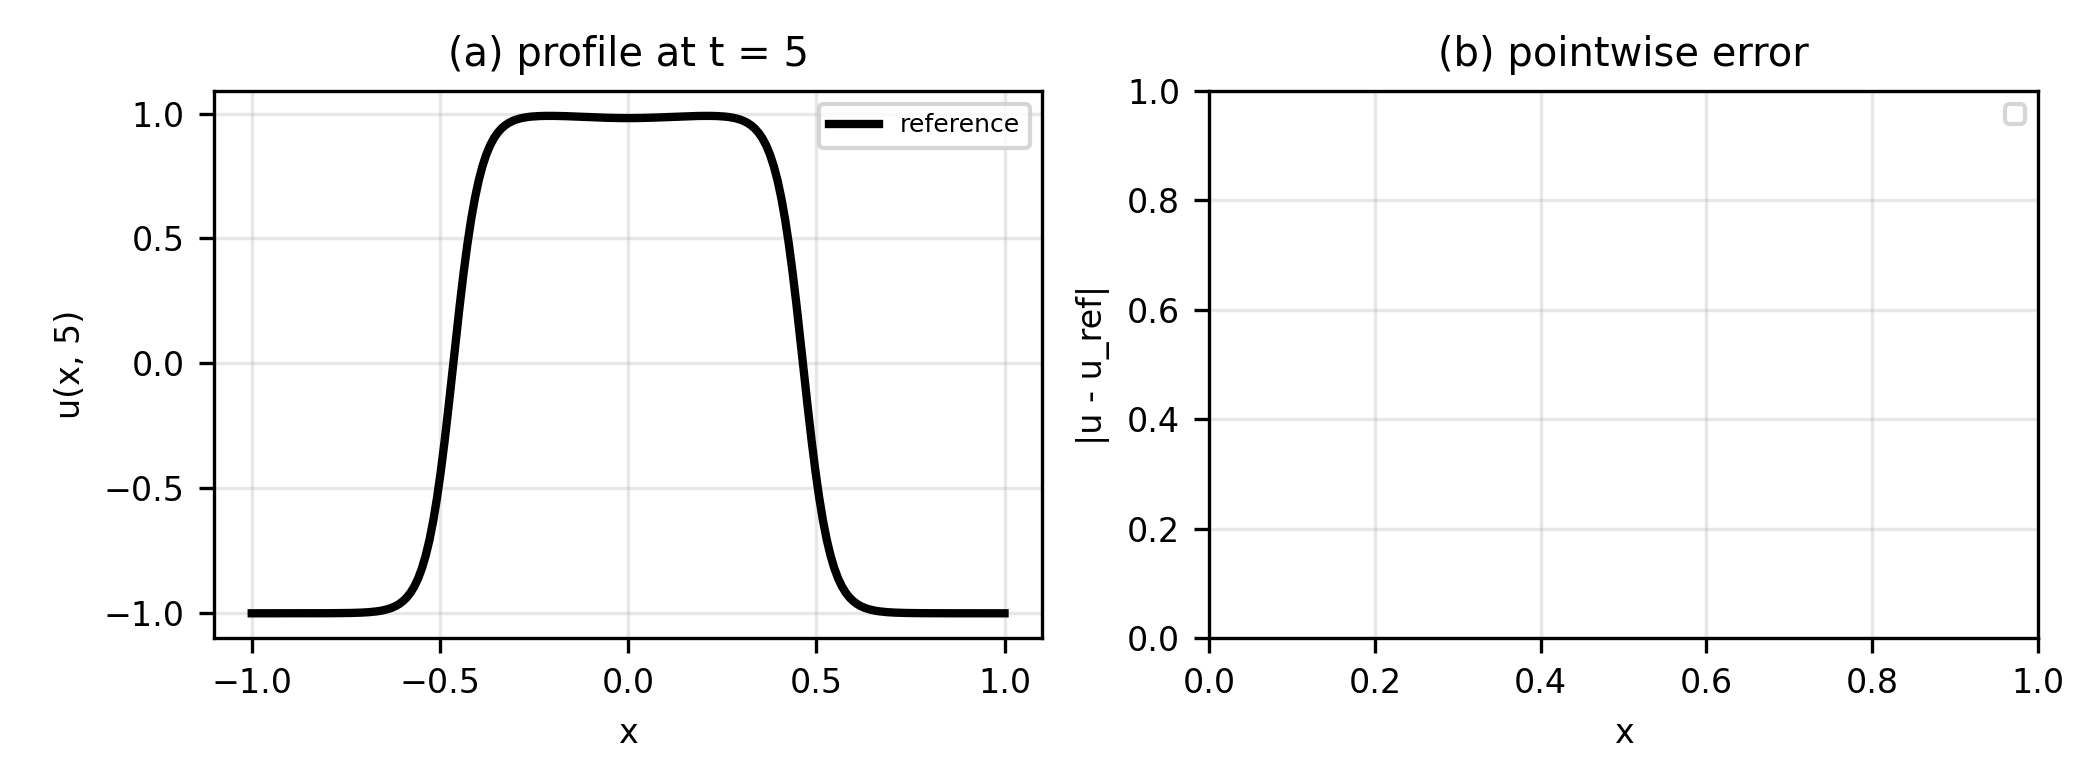
\includegraphics[width=\textwidth]{figures_r1/fig_b3.png}
\caption{\rev{Benchmark B3 ($\varepsilon=0.05$, $T=5$): (a) profiles at $t=5$ of the certified reference and of trained networks (seed 42), (b) pointwise error.}\label{fig:b3}}
\end{figure}


\subsection{Mode Number: the Previously Reported Degradation Was a Boundary-Penalty Artefact}\label{sec:results-k}

\rev{The first version reported that the accuracy of the Spectral-PINN \emph{degrades} as the number of Chebyshev modes $K$ grows, even when the training budget is scaled with $K$, and interpreted this as an optimization bottleneck specific to the coefficient parameterization. This was wrong. In that code the Neumann penalty was applied to $u_x(\pm1,t)/K^2$ and then squared, so its effective weight on $u_x(\pm1)^2$ was $\lambda_{\rm BC}K^{-4}$, i.e.\ it vanished as $K$ grew: the trained $K=64$ network of the as-submitted variant has wall slopes $|u_x(\pm1)|$ up to \N{kk.soft64.wall} instead of zero, and the PDE solution cannot be matched with such a polynomial. Table~\ref{tab:K} separates the factors. With the exact Neumann basis the $L^2$ error at $K=64$ is \N{kk.hard64.l2} (five seeds), compared with \N{kk.soft64.l2} for the as-submitted variant; at $K=128$ the numbers are \N{kk.hard128.l2} and \N{kk.soft128.l2}. Rescaling the soft penalty so that its effective weight is $1$ ($\lambda_{\rm BC}=K^4$) also removes the degradation (\N{kk.fix64.l2} at $K=64$), which shows that it is the missing boundary enforcement, and not the soft constraint as such, that was responsible. The grid has a secondary effect (Gauss--Lobatto instead of equispaced collocation improves the soft variant at $K=64$ by a factor \N{kk.cgl_soft_gain}). With the revised variant the error changes only mildly with $K$ (\N{kk.hard32.l2} at $K=32$, \N{kk.hard64.l2} at $K=64$, \N{kk.hard128.l2} at $K=128$), and the runs with larger budgets and with $K=256$ are listed in Table~\ref{tab:K}.}

\begin{table}[H]
\caption{\rev{Effect of the mode number $K$ for different treatments of the Neumann condition and of the collocation grid (B1, $L^2$ error at $t=1$). Budget is the number of epochs relative to $6000+1000$ warm-up epochs. Single-seed rows have $n=1$ (SD not defined). The wall slope is the maximum of $|u_x(\pm1,t)|$ over the trained trajectory. Times marked $^\dagger$ come from concurrently executed runs.}\label{tab:K}}
\small
\begin{tabularx}{\textwidth}{p{4.8cm}cccccc}
\toprule
\textbf{Variant} & $K$ & Budget & $L^2$ error & max $|u_x(\pm1)|$ & $n$ & Time (s)\\
\midrule
soft penalty, equispaced grid (as submitted) & 32 & $1\times$ & \textbf{--} & \textbf{--} & 0 & \textbf{--}\\
 & 64 & $1\times$ & \ensuremath{(9.93\pm1.56)\times10^{-2}} & 5.67 & 4 & 410$^\dagger$\\
 & 128 & $1\times$ & \textbf{--} & \textbf{--} & 0 & \textbf{--}\\
soft penalty, Gauss--Lobatto grid & 32 & $1\times$ & \ensuremath{9.33\times10^{-4}} & 0.55 & 1 & 192$^\dagger$\\
 & 64 & $1\times$ & \ensuremath{1.52\times10^{-2}} & 4.02 & 1 & 446$^\dagger$\\
soft penalty rescaled ($\lambda_{\rm BC}=K^4$) & 32 & $1\times$ & \textbf{--} & \textbf{--} & 0 & \textbf{--}\\
 & 64 & $1\times$ & \textbf{--} & \textbf{--} & 0 & \textbf{--}\\
 & 128 & $1\times$ & \textbf{--} & \textbf{--} & 0 & \textbf{--}\\
\midrule
exact Neumann basis, equispaced grid & 64 & $1\times$ & \ensuremath{2.07\times10^{-3}} & 0.00 & 1 & 475$^\dagger$\\
exact Neumann basis, Gauss--Lobatto grid (revised) & 32 & $1\times$ & \ensuremath{(8.29\pm1.43)\times10^{-4}} & 0.00 & 5 & 251$^\dagger$\\
 & 64 & $1\times$ & \ensuremath{(1.46\pm0.42)\times10^{-3}} & 0.00 & 5 & 587$^\dagger$\\
 & 128 & $1\times$ & \ensuremath{(6.57\pm1.80)\times10^{-3}} & 0.00 & 2 & 732$^\dagger$\\
 & 64 & $2\times$ & \textbf{--} & \textbf{--} & 0 & \textbf{--}\\
 & 128 & $2\times$ & \textbf{--} & \textbf{--} & 0 & \textbf{--}\\
 & 256 & $1\times$ & \textbf{--} & \textbf{--} & 0 & \textbf{--}\\
\bottomrule
\end{tabularx}

\end{table}


\begin{figure}[H]
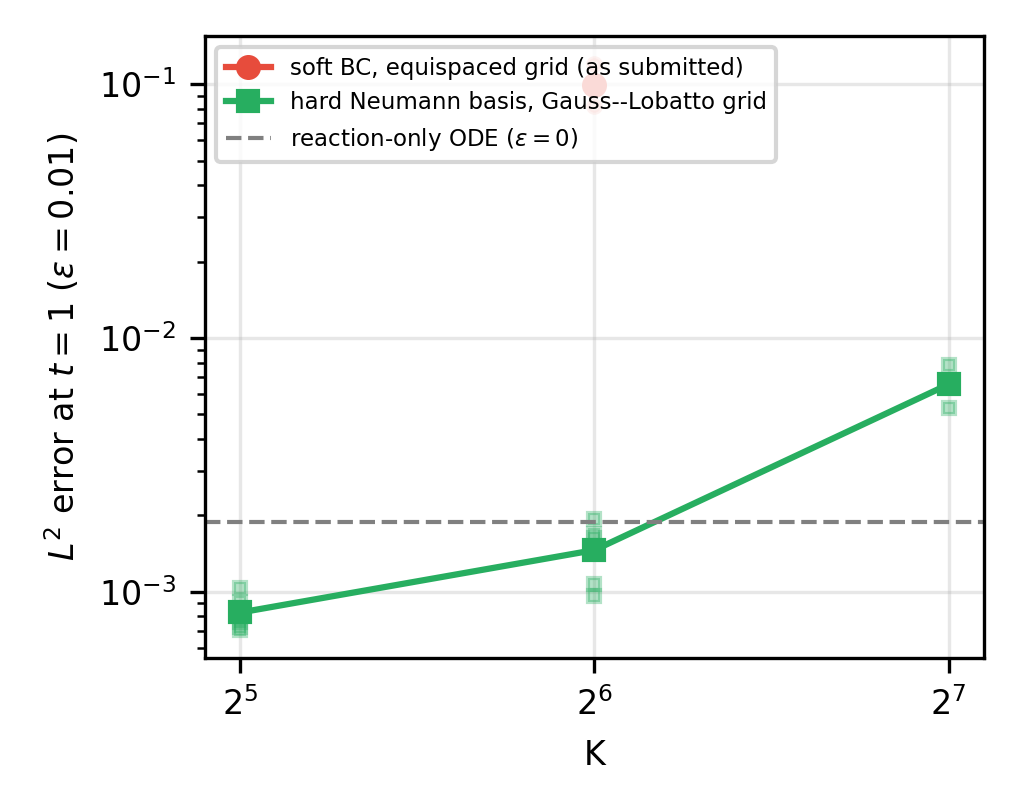
\includegraphics[width=8.5cm]{figures_r1/fig_K.png}
\caption{\rev{$L^2$ error at $t=1$ of the as-submitted (soft Neumann penalty, equispaced collocation) and the revised (exact Neumann basis, Gauss--Lobatto collocation) Spectral-PINN versus the mode number $K$ (B1; small symbols: individual seeds, large: mean). The dashed line is the error of the reaction-only model.}\label{fig:K}}
\end{figure}

\subsection{Energy Penalty: Weight, Regimes and the Energy Curves}\label{sec:results-energy}

\rev{The weight of the energy penalty in all runs of the first version was $\lambda_E=50$ (it was not reported there); the penalty acts on $10$ checkpoints per unit time. In B1 the unpenalized network already decreases its energy at every one of the $50$ intervals of a grid with spacing $0.02$ (and at every interval of the grids with spacing $0.002$ and $2\times10^{-4}$) in all \N{en.n_runs} runs of the revised $K=32$ network, with or without the penalty; the energy changes by at least \N{en.min_step} per interval of length $0.02$, whereas the penalty changes the energy trajectory by at most \N{en.max_diff}, which is why the two curves of Figure~\ref{fig:energy}(a) coincide: in this regime the penalty has no effect that one can see, and the zero violations reported in the first version cannot be attributed to it. The penalty term itself is positive in at most \N{en.nonzero} of the 6000 training epochs at $\lambda_E=50$ (over five seeds). Table~\ref{tab:energy} varies $\lambda_E$ from $0$ to $5000$: neither the accuracy nor the number of energy increases depends on it (the accuracy is within one seed-to-seed standard deviation for every value). We also looked for regimes in which the unpenalized trajectory is poor: a training run cut to 300 epochs, no warm-up, and a ten times smaller learning rate (Table~\ref{tab:energy}, lower part). \TODO{describe what Table~\ref{tab:energy} shows for these regimes once the group regimes\_hard has been run: does the penalty change the count of energy increases or the error? Do not claim more than the table shows.}}

\begin{table}[H]
\caption{\rev{Energy penalty weight and regime (revised Spectral-PINN, $K=32$, B1). ``increases'' is the total number of energy increases (more than $10^{-10}$) over all seeds on grids of spacing $0.02$, $0.002$, $2\times10^{-4}$; ``penalty $>0$'' is the largest number, over the seeds, of training epochs at which $\mathcal L_E>0$ (out of the total number of epochs).}\label{tab:energy}}
\small
\begin{tabularx}{\textwidth}{p{4.6cm}cccc}
\toprule
Setting & $n$ & $L^2$ error at $t=1$ & increases (0.02 / 0.002 / $2\times10^{-4}$) & penalty $>0$ in epochs\\
\midrule
$\lambda_E=0$ & 5 & \ensuremath{(8.29\pm1.43)\times10^{-4}} & 0 / 0 / 0 & 0\\
$\lambda_E=1$ & 0 & \textbf{--} & \textbf{--} & \textbf{--}\\
$\lambda_E=10$ & 0 & \textbf{--} & \textbf{--} & \textbf{--}\\
$\lambda_E=50$ & 5 & \ensuremath{(8.29\pm1.45)\times10^{-4}} & 0 / 0 / 0 & 1\\
$\lambda_E=500$ & 0 & \textbf{--} & \textbf{--} & \textbf{--}\\
$\lambda_E=5000$ & 0 & \textbf{--} & \textbf{--} & \textbf{--}\\
\midrule
300 epochs, warm-up 100, $\lambda_E=0$ & 0 & \textbf{--} & \textbf{--} & \textbf{--}\\
300 epochs, warm-up 100, $\lambda_E=50$ & 0 & \textbf{--} & \textbf{--} & \textbf{--}\\
no warm-up, $\lambda_E=0$ & 0 & \textbf{--} & \textbf{--} & \textbf{--}\\
no warm-up, $\lambda_E=50$ & 0 & \textbf{--} & \textbf{--} & \textbf{--}\\
learning rate $10^{-4}$, 1500 epochs, $\lambda_E=0$ & 0 & \textbf{--} & \textbf{--} & \textbf{--}\\
learning rate $10^{-4}$, 1500 epochs, $\lambda_E=50$ & 0 & \textbf{--} & \textbf{--} & \textbf{--}\\
\bottomrule
\end{tabularx}

\end{table}


\begin{figure}[H]
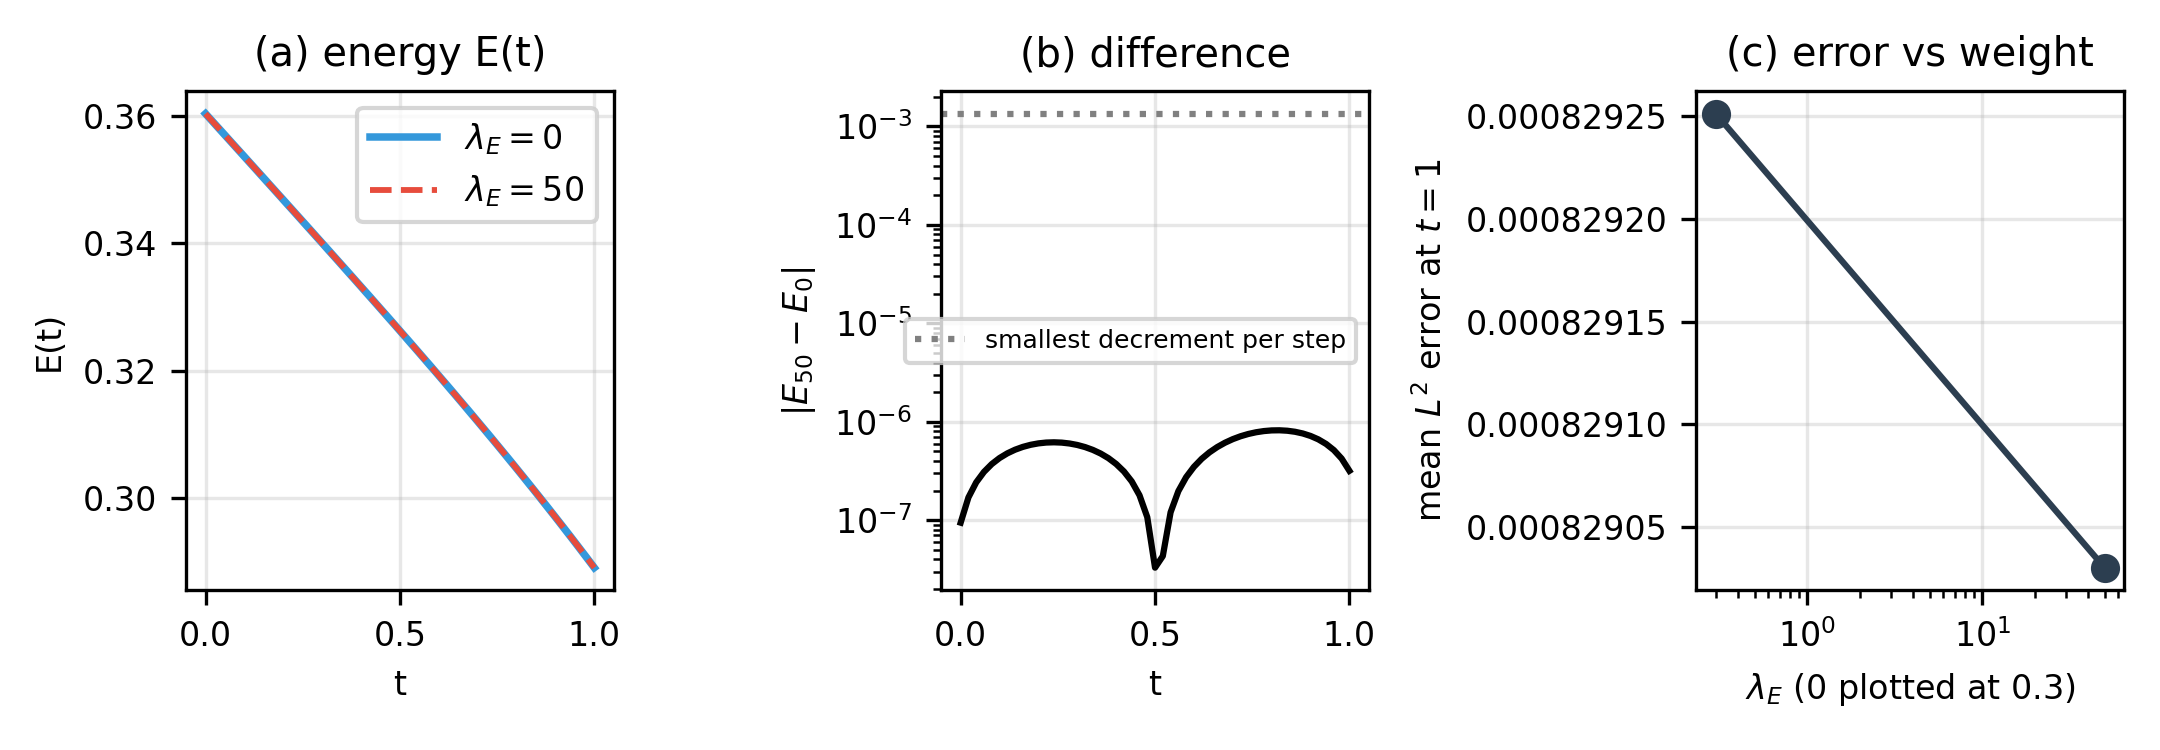
\includegraphics[width=\textwidth]{figures_r1/fig_energy.png}
\caption{\rev{Energy of the trained trajectory (B1, $K=32$, seed 42) with and without the energy penalty: (a) $E(t)$; (b) the absolute difference of the two curves compared with the smallest decrement of $E$ per grid interval; (c) mean $L^2$ error versus $\lambda_E$ (five seeds).}\label{fig:energy}}
\end{figure}

\subsection{Maximum Bound Principle and the A-Posteriori Energy Balance}\label{sec:results-balance}

\rev{\emph{Maximum bound.} The exact solution satisfies $|u|\le1$ (the certified reference has $\max|u|=0.9998$ at $t=1$); decreasing energy does not imply this~\cite{ref_Du2021b,ref_He2019}. We therefore report $\max_{x,t}|u_\theta|$ for every trained network (Table~\ref{tab:forward}). The Spectral-PINN overshoots slightly in all runs: the largest value over all B1 runs is \N{mbp.max_b1} (the revised variant: \N{mbp.max_hard}), i.e.\ the bound is respected to \N{mbp.excess}, which is of the order of the approximation error, but it is \emph{not} guaranteed, and the overshoot occurs on the plateaus $u\approx\pm1$ where the network has the least ability to resolve $\tanh$-type tails with a polynomial. The vanilla PINN overshoots more (\N{mbp.max_van}). A guaranteed bound would require a limiter as in~\cite{ref_Geng2025}; we do not attempt one.}

\rev{\emph{Energy balance.} For every trained network we evaluated the identity~\eqref{eq:balance-main} and the bound~\eqref{eq:balance-int} (Table~\ref{tab:balance}). The identity holds to round-off (relative error \N{bal.id_err}), which checks the code against the proposition. The time-integrated residual $\frac12\int_0^T\|r\|^2dt$ is \N{bal.int_r_hard} for the revised $K=32$ network (B1), against an actual energy decrease $E(0)-E(T)=\N{bal.dE_hard}$; thus the energy of the learned solution cannot increase between two times by more than \N{bal.int_r_hard}, a small fraction (\N{bal.frac_hard}) of its decrease, and it is $\|u_t\|^2$ rather than the residual that drives the decay. For the as-submitted $K=64$ network the boundary defect adds \N{bal.int_b_soft}. Figure~\ref{fig:balance}(a) compares both sides of the identity along the trained trajectory, and Figure~\ref{fig:balance}(b) the residual of the trained networks.}

\begin{table}[H]
\caption{\rev{A-posteriori energy balance of the trained trajectories (Section~\ref{sec:balance}): wall slope, time-integrated residual $\frac12\int_0^T\|r\|^2dt$, time-integrated boundary defect, actual energy decrease, and relative error of the identity~\eqref{eq:balance-main} checked against the autograd derivative of $E(t)$ (maximum over seeds). Means over seeds.}\label{tab:balance}}
\small
\begin{tabularx}{\textwidth}{Xcccccc}
\toprule
\textbf{Network} & $n$ & max $|u_x(\pm1)|$ & $\frac12\!\int\!\|r\|^2$ & $\int|\beta|$ & $E(0)-E(T)$ & id. error\\
\midrule
revised $K=32$ & 5 & 3.6e-15 & \ensuremath{1.28\times10^{-5}} & \ensuremath{3.72\times10^{-22}} & 0.071 & \ensuremath{3.4\times10^{-16}}\\
revised $K=32$, $\lambda_E=50$ & 5 & 3.6e-15 & \ensuremath{1.28\times10^{-5}} & \ensuremath{4.12\times10^{-22}} & 0.071 & \ensuremath{3.4\times10^{-16}}\\
revised $K=64$ & 5 & 4.4e-15 & \ensuremath{2.08\times10^{-5}} & \ensuremath{4.01\times10^{-22}} & 0.071 & \ensuremath{3.4\times10^{-16}}\\
revised $K=128$ & 2 & 7.1e-15 & \ensuremath{5.86\times10^{-5}} & \ensuremath{1.94\times10^{-21}} & 0.070 & \ensuremath{3.4\times10^{-16}}\\
as submitted $K=64$ & 4 & 5.7e+00 & \ensuremath{4.57\times10^{-4}} & \ensuremath{4.11\times10^{-6}} & 0.058 & \ensuremath{4.4\times10^{-16}}\\
revised, B2 & 0 & \textbf{--} & \textbf{--} & \textbf{--} & \textbf{--} & \textbf{--}\\
revised $K=64$, B3 & 0 & \textbf{--} & \textbf{--} & \textbf{--} & \textbf{--} & \textbf{--}\\
\bottomrule
\end{tabularx}

\end{table}


\begin{figure}[H]
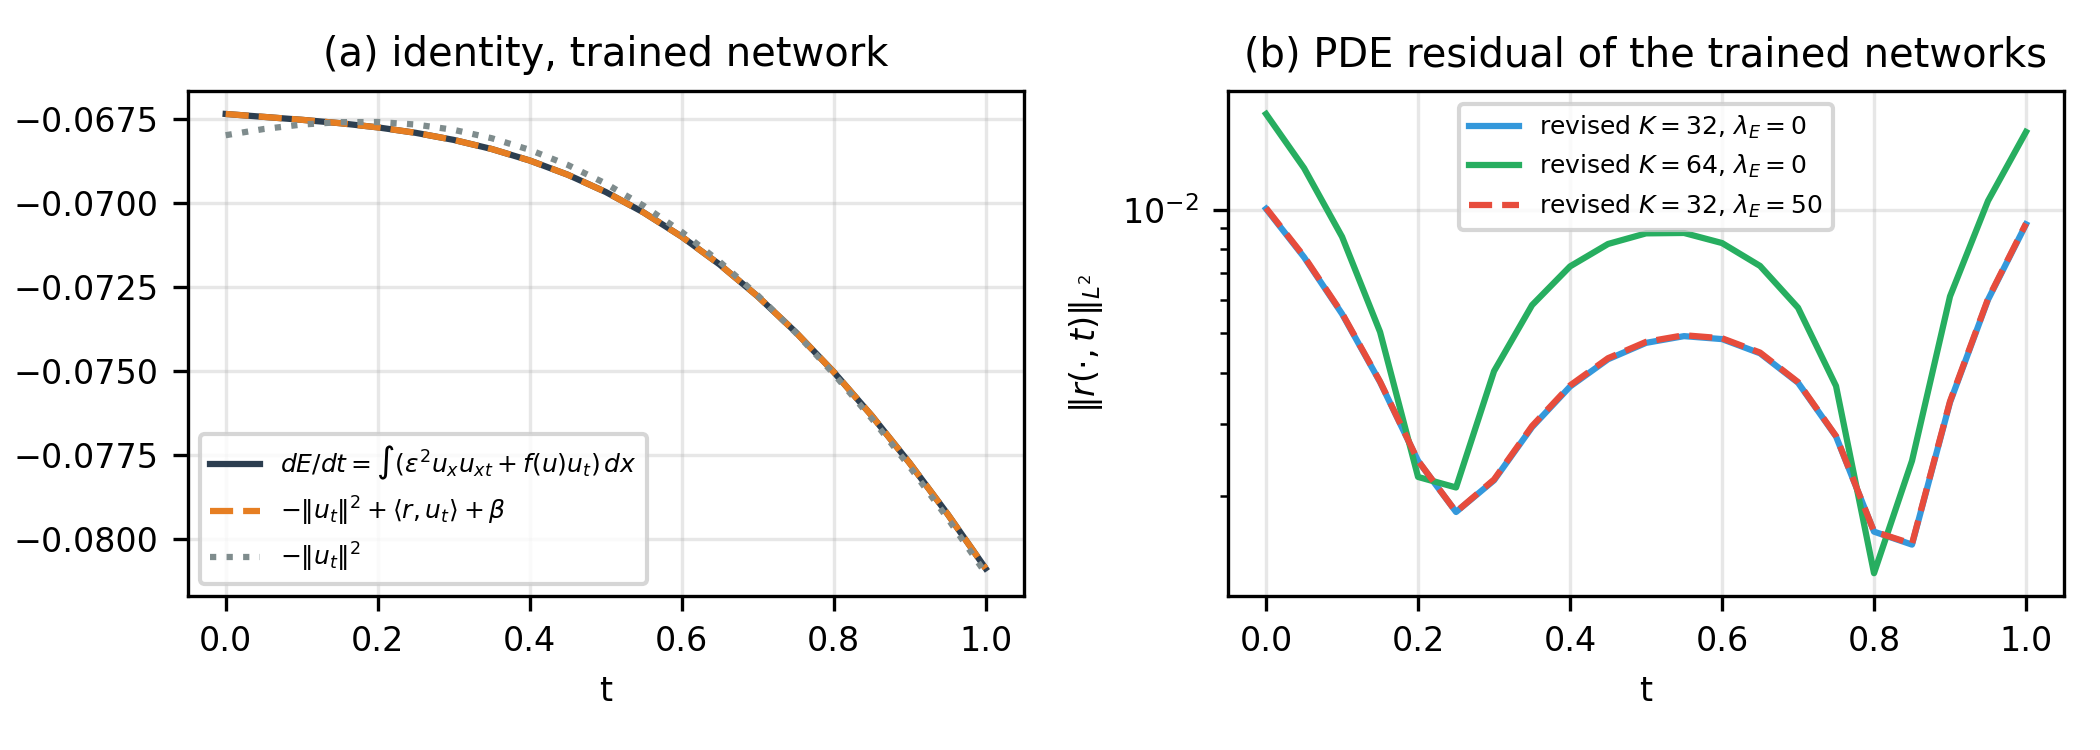
\includegraphics[width=\textwidth]{figures_r1/fig_balance.png}
\caption{\rev{(a) The two sides of the energy identity~\eqref{eq:balance-main} along the trained trajectory (B1, $K=32$, $\lambda_E=50$, seed 42): they coincide to round-off. (b) $L^2$ norm of the PDE residual versus time for trained networks.}\label{fig:balance}}
\end{figure}

\subsection{Inverse Problem}\label{sec:results-inverse}

\rev{\emph{What the first version reported, and why it was wrong.} The first version reported a ``robust $\sim38\%$ overestimation bias'' of the recovered $\varepsilon$ and attributed it to the loss weighting, the warm-up or the observation design, without an ablation. We now show that the number $38\%$ is not a property of the estimator but the footprint of the starting value. With the joint-Adam procedure of Section~\ref{sec:inverse} the recovered value satisfies $\hat\varepsilon/\varepsilon_{\rm init}\in[\N{inv.ratio_range}]$ for every starting value $\varepsilon_{\rm init}\in\{0.5,1,1.5,2,4\}\,\varepsilon_{\rm true}$ and for $\varepsilon_{\rm true}\in\{0.05,0.1\}$ (Figure~\ref{fig:inverse}(a), Table~\ref{tab:inverse1}); the first version had always used $\varepsilon_{\rm init}=2\varepsilon_{\rm true}$, and $0.717\times2=1.43$ is the ``bias''. The data enter only weakly: the estimate is the same for $\lambda_{\rm data}=2$ and $2000$, for 10, 40 and 160 observation points, for 5 and 20 snapshots and for $K=16,32,64$ (Table~\ref{tab:inverse2}), and it started from the true value moves away from it. The mechanism is the optimizer: Adam moves $\log\varepsilon$ by about $\pm$ the learning rate per step while the sign of the gradient is consistent, and after $\approx\N{inv.steps}$ steps the gradient signal (which is tiny compared with the early transient of the network) is swamped by the second-moment memory and the parameter freezes; changing the learning-rate multiplier of $\log\varepsilon$ by a factor $10^{\pm2}$ changes the total displacement by the same factor, in line with this explanation. The estimates reported in the first version for the noise experiments ($40.2$, $40.2$, $40.0\%$) and for a single run at $\varepsilon_{\rm true}=0.05$ ($14.7\%$) came from a script whose settings differed from those stated and whose output was not archived; they are withdrawn.}

\rev{\emph{An estimator that does not depend on the start.} Because the residual is linear in $\varepsilon^2$, the optimal $\varepsilon^2$ for a given network is available in closed form (variable projection, Section~\ref{sec:inverse}). Combined with a data-fitting phase and a large data weight it recovers $\varepsilon$ from noise-free data with relative errors of \N{inv.vp_err_005} ($\varepsilon_{\rm true}=0.05$) and \N{inv.vp_err_01} ($\varepsilon_{\rm true}=0.1$) at $\lambda_{\rm data}=2000$ (Figure~\ref{fig:inverse}(b); the error falls with $\lambda_{\rm data}$ because the accuracy of the data fit has to be much smaller than the signal carried by $\varepsilon$). The classical least-squares estimator with the Chebyshev solver recovers the exact value in the noise-free case by construction (inverse crime) and is the benchmark in the noisy case.}

\begin{table}[H]
\caption{\rev{Joint Adam training of the network and $\log\varepsilon$ (as in the first version): recovered $\hat\varepsilon$ for different starting values $\varepsilon_{\rm init}$ (noise-free data, 5 snapshots, 40 points, $\lambda_{\rm data}=2$, one run each). The ratio to the starting value is nearly constant, and data and truth have little influence.}\label{tab:inverse1}}
\small
\begin{tabularx}{\textwidth}{cccccc}
\toprule
$\varepsilon_{\rm init}/\varepsilon_{\rm true}$ & variant & $\varepsilon_{\rm true}$ & $\hat\varepsilon/\varepsilon_{\rm true}$ & $\hat\varepsilon/\varepsilon_{\rm init}$ & data misfit (RMS)\\
\midrule
0.5 & as submitted & 0.05 & 0.36 & 0.72 & 2.8e-02\\
0.5 & revised & 0.05 & 0.31 & 0.61 & 7.9e-03\\
1 & as submitted & 0.05 & 0.71 & 0.71 & 5.1e-02\\
1 & revised & 0.05 & 0.68 & 0.68 & 6.7e-03\\
1.5 & as submitted & 0.05 & 1.08 & 0.72 & 6.7e-02\\
1.5 & revised & 0.05 & 1.10 & 0.73 & 7.8e-03\\
2 & as submitted & 0.05 & 1.43 & 0.72 & 8.2e-02\\
2 & revised & 0.05 & 1.37 & 0.69 & 1.4e-02\\
4 & as submitted & 0.05 & 2.87 & 0.72 & 1.3e-01\\
4 & revised & 0.05 & 2.73 & 0.68 & 5.1e-02\\
0.5 & soft & 0.1 & \textbf{--} & \textbf{--} & \textbf{--}\\
0.5 & hard & 0.1 & \textbf{--} & \textbf{--} & \textbf{--}\\
1 & soft & 0.1 & \textbf{--} & \textbf{--} & \textbf{--}\\
1 & hard & 0.1 & \textbf{--} & \textbf{--} & \textbf{--}\\
1.5 & soft & 0.1 & \textbf{--} & \textbf{--} & \textbf{--}\\
1.5 & hard & 0.1 & \textbf{--} & \textbf{--} & \textbf{--}\\
2 & soft & 0.1 & \textbf{--} & \textbf{--} & \textbf{--}\\
2 & hard & 0.1 & \textbf{--} & \textbf{--} & \textbf{--}\\
4 & soft & 0.1 & \textbf{--} & \textbf{--} & \textbf{--}\\
4 & hard & 0.1 & \textbf{--} & \textbf{--} & \textbf{--}\\
\bottomrule
\end{tabularx}

\end{table}

\begin{table}[H]
\caption{\rev{Variable-projection estimator: noise-free data, effect of the data weight (upper part) and of the observation design and loss weights (lower part, $\varepsilon_{\rm true}=0.05$).}\label{tab:inverse2}}
\small
\begin{tabularx}{\textwidth}{Xcccc}
\toprule
Setting & $n$ & $\varepsilon_{\rm true}$ & rel. error of $\hat\varepsilon$ (\%) & data misfit (RMS)\\
\midrule
variable projection, $\lambda_{\rm data}=20$ & 0 & 0.05 & \textbf{--} & \textbf{--}\\
variable projection, $\lambda_{\rm data}=200$ & 0 & 0.05 & \textbf{--} & \textbf{--}\\
variable projection, $\lambda_{\rm data}=2000$ & 0 & 0.05 & \textbf{--} & \textbf{--}\\
variable projection, $\lambda_{\rm data}=20000$ & 0 & 0.05 & \textbf{--} & \textbf{--}\\
variable projection, $\lambda_{\rm data}=20$ & 0 & 0.1 & \textbf{--} & \textbf{--}\\
variable projection, $\lambda_{\rm data}=200$ & 0 & 0.1 & \textbf{--} & \textbf{--}\\
variable projection, $\lambda_{\rm data}=2000$ & 0 & 0.1 & \textbf{--} & \textbf{--}\\
variable projection, $\lambda_{\rm data}=20000$ & 0 & 0.1 & \textbf{--} & \textbf{--}\\
\midrule
10 observation points, $\lambda_{\rm data}=2000$ & 0 & 0.05 & \textbf{--} & \textbf{--}\\
160 observation points, $\lambda_{\rm data}=2000$ & 0 & 0.05 & \textbf{--} & \textbf{--}\\
3 snapshots, $\lambda_{\rm data}=2000$ & 0 & 0.05 & \textbf{--} & \textbf{--}\\
20 snapshots, $\lambda_{\rm data}=2000$ & 0 & 0.05 & \textbf{--} & \textbf{--}\\
$\lambda_{\rm PDE}=5$, $\lambda_{\rm data}=2000$ & 0 & 0.05 & \textbf{--} & \textbf{--}\\
$\lambda_{\rm PDE}=500$, $\lambda_{\rm data}=2000$ & 0 & 0.05 & \textbf{--} & \textbf{--}\\
no data-fitting phase, $\lambda_{\rm data}=2000$ & 0 & 0.05 & \textbf{--} & \textbf{--}\\
$K=64$, $\lambda_{\rm data}=2000$ & 0 & 0.05 & \textbf{--} & \textbf{--}\\
\bottomrule
\end{tabularx}

\end{table}

\begin{table}[H]
\caption{\rev{Inverse problem with noisy data: neural variable-projection estimator (5 noise realizations; $\lambda_{\rm data}=2000$) against the classical least-squares estimator with the Chebyshev solver (20 realizations) and the Cram\'er--Rao bound $\sigma/\|\partial_{\log\varepsilon}\mathbf d\|$. At $\varepsilon=0.01$ the problem is not identifiable for $\sigma\ge0.01$.}\label{tab:inverse3}}
\small
\begin{tabularx}{\textwidth}{ccXcc}
\toprule
$\varepsilon_{\rm true}$ & $\sigma$ & neural (variable projection): mean $|$rel. err.$|$ (\%) & classical LS: RMSE (\%) & Cram\'er--Rao (\%)\\
\midrule
0.05 & 0.01 & \textbf{--} & 2.6 & 2.0\\
0.05 & 0.05 & \textbf{--} & 8.8 & 10.2\\
0.1 & 0.01 & \textbf{--} & 0.7 & 0.7\\
0.1 & 0.05 & \textbf{--} & 2.6 & 3.4\\
0.01 & 0 & \textbf{--} & 0.0 & 0.0\\
0.01 & 0.01 & \textbf{--} & 53.2 & 45.4\\
\bottomrule
\end{tabularx}

\end{table}


\begin{figure}[H]
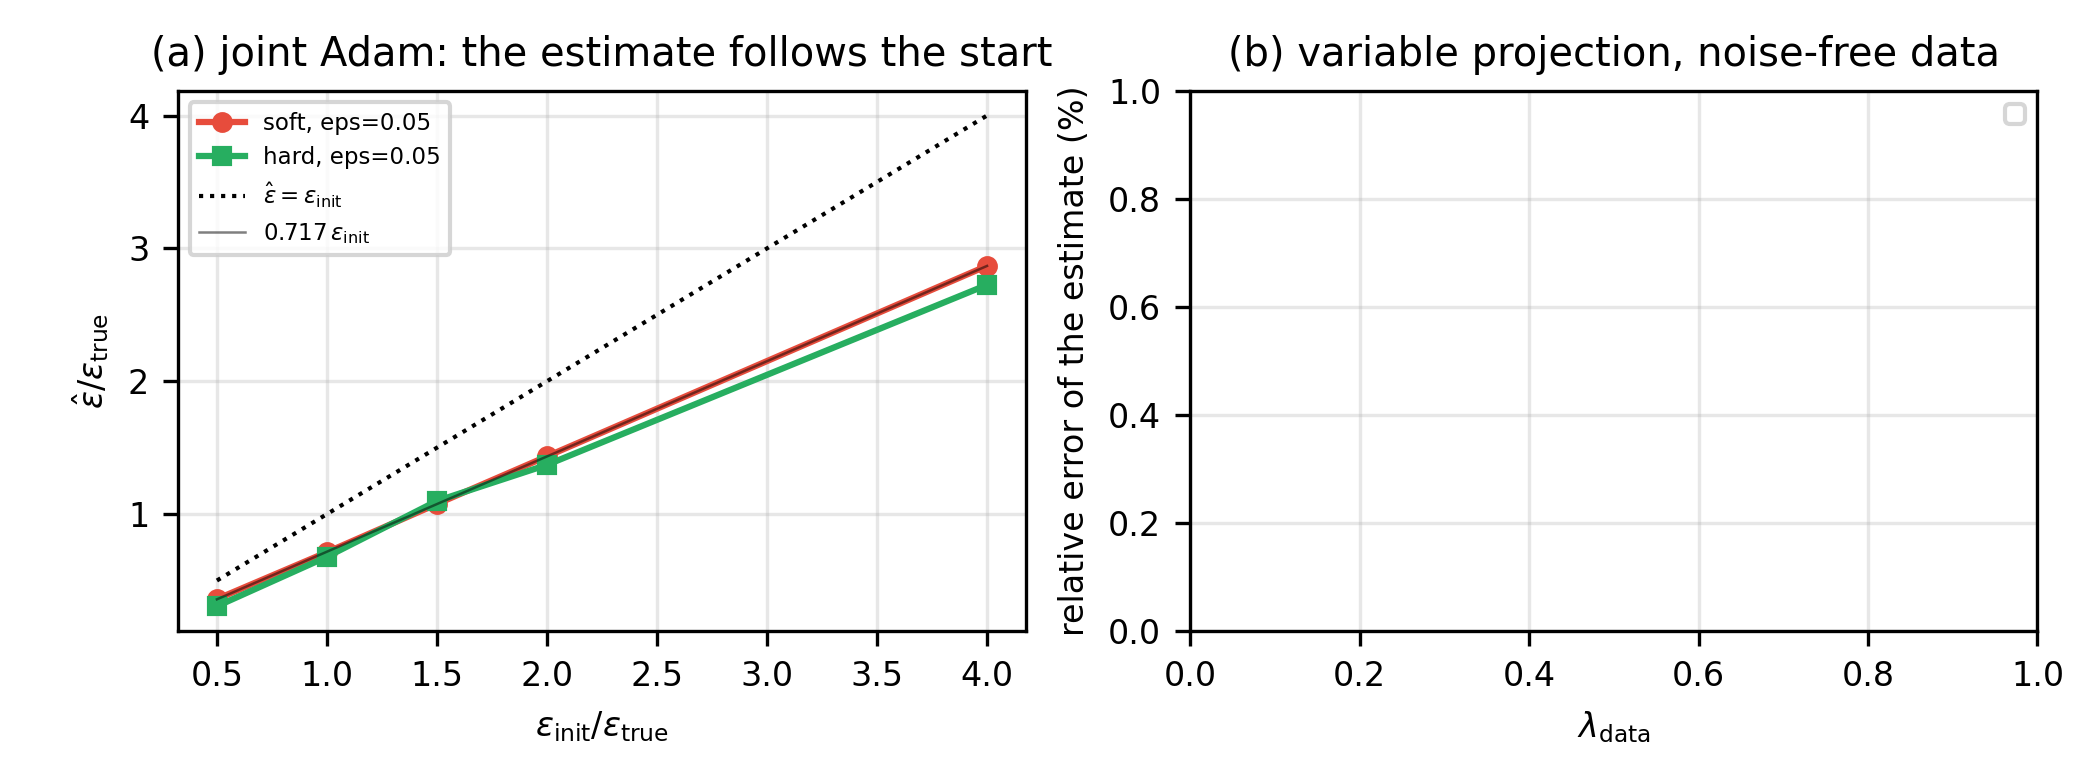
\includegraphics[width=\textwidth]{figures_r1/fig_inverse.png}
\caption{\rev{(a) Joint Adam: ratio $\hat\varepsilon/\varepsilon_{\rm true}$ versus the starting value; both the as-submitted and the revised network follow $\approx0.72\,\varepsilon_{\rm init}$ (dotted: no change). (b) Variable projection: relative error versus the data weight, noise-free data.}\label{fig:inverse}}
\end{figure}

\rev{\emph{Identifiability.} The data constrain $\varepsilon$ only through the term $\varepsilon^2u_{xx}$, which is small on this benchmark. For the observation design of this study (40 points, 5 times) the norm of the derivative of the data vector with respect to $\log\varepsilon$ is \N{ident.S001} at $\varepsilon=0.01$, \N{ident.S005} at $0.05$ and \N{ident.S01} at $0.1$. With Gaussian noise of standard deviation $\sigma=0.01$ the Cram\'er--Rao standard error of $\log\hat\varepsilon$ is therefore \N{ident.se001} at $\varepsilon=0.01$, and the classical least-squares estimator indeed has an error of \N{ident.cl001} there, while at $\varepsilon=0.05$ it is \N{ident.cl005}. For $\varepsilon=0.01$ no estimator can recover $\varepsilon$ from $\sigma\ge0.01$ data; the ``inverse problem at $\varepsilon=0.01$'' of the first version was therefore not a meaningful test. Table~\ref{tab:inverse3} compares the neural and the classical estimator under noise.}

\subsection{Two-Dimensional Symmetry Preservation}\label{sec:2d-results}

\rev{The two-dimensional results are unchanged from the first version (the experiment does not involve a Neumann condition) and the statements are corrected.} Table~\ref{tab:2d} gives the reflection-symmetry violation $S(t)$. The Fourier-Spectral-PINN stays at round-off, $S\in[\N{s2d.fmin},\N{s2d.fmax}]$ for $t\in[0,1]$, independently of the seed, while the vanilla PINN with the same periodic encoding has $S$ increasing monotonically in every one of the five seeds, by a factor of \N{s2d.growth} (individual seeds: \N{s2d.growth_range}) between $t=0$ and $t=1$. \rev{Larger mode counts and a sharper interface do not change this (Table~\ref{tab:stress-2d}): at $t=1$ the violation stays between \N{s2d.smin} and \N{s2d.smax} in all five configurations, i.e.\ at the level of round-off (the corresponding RMS asymmetry is $6\times10^{-16}$ at the largest value, about three times the machine epsilon); it is about three times larger for $\varepsilon=0.1$ than for $\varepsilon=0.3$, because the energy of the field is larger, not because the symmetry is only approximate. The training budget was doubled in two of the three $M=16$ runs.}

\begin{table}[H]
\caption{Reflection-symmetry violation $S(t)$ (Section~\ref{sec:2d}) for the Fourier-Spectral-PINN (single run; architecturally exact regardless of seed) versus a vanilla PINN with the same periodic input encoding (mean $\pm$ SD over 5 seeds). Data of the first version, unchanged.\label{tab:2d}}
\small
\begin{tabularx}{\textwidth}{ccc}
\toprule
$t$ & Fourier-Spectral-PINN & Vanilla PINN (5 seeds)\\
\midrule
0.0 & \ensuremath{8.71\times10^{-32}} & \ensuremath{(4.12\pm1.13)\times10^{-5}}\\
0.2 & \ensuremath{9.41\times10^{-32}} & \ensuremath{(4.94\pm1.16)\times10^{-5}}\\
0.5 & \ensuremath{1.03\times10^{-31}} & \ensuremath{(9.46\pm1.81)\times10^{-5}}\\
1.0 & \ensuremath{1.26\times10^{-31}} & \ensuremath{(2.22\pm0.45)\times10^{-4}}\\
\bottomrule
\end{tabularx}

\end{table}

\begin{table}[H]
\caption{Fourier-Spectral-PINN reflection-symmetry violation $S(1)$ at larger $M$ and smaller $\varepsilon$ (data of the first version, unchanged).\label{tab:stress-2d}}
\small
\begin{tabularx}{\textwidth}{cccc}
\toprule
$M$ & $\varepsilon$ & epochs & $S(1)$\\
\midrule
8 & 0.3 & 3000 & \ensuremath{1.27\times10^{-31}}\\
16 & 0.3 & 3000 & \ensuremath{1.27\times10^{-31}}\\
16 & 0.3 & 6000 & \ensuremath{1.26\times10^{-31}}\\
8 & 0.1 & 3000 & \ensuremath{3.74\times10^{-31}}\\
16 & 0.1 & 6000 & \ensuremath{3.74\times10^{-31}}\\
\bottomrule
\end{tabularx}

\end{table}

%%%%%%%%%%%%%%%%%%%%%%%%%%%%%%%%%%%%%%%%%%
\section{Discussion}

\subsection{What the Coefficient-Space Network Does and Does Not Achieve}\label{sec:niche}

\rev{On the forward problem the answer to the question of whether a PINN can compete with a classical spectral solver is, in this study, no: on B1 and B2 Chebyshev collocation with an ordinary first-order time step is \N{b1.ratio.fh_K32_cheb80} times more accurate and several orders of magnitude cheaper than the best Spectral-PINN, and the reaction-only model is as accurate as the network on B1. This agrees with the established outcome for forward problems~\cite{ref_Grossmann2024,ref_McGreivy2024} and we do not offer the method as a competitor on this task. What the experiments do show is narrower: (i)~inside the family of PINNs, putting the discretization into the output space removes the need for spatial automatic differentiation and gives a gain of \N{b1.ratio.van_fhK32} in accuracy and about \N{b1.speed.van_fhK32} in cost over the space--time PINN on B1 (and the vanilla PINN still has an error of \N{b1.lb_van.l2} after an L-BFGS stage); (ii)~structure that is a linear constraint on the coefficients can be imposed exactly (the Neumann basis~\eqref{eq:neumann-basis}, or the reflection-symmetric Fourier basis of Section~\ref{sec:2d-results}) at no cost in accuracy, and doing so removed a failure that a penalty produced (Section~\ref{sec:results-k}); (iii)~the energy of the learned trajectory is controlled a posteriori by quantities that can be computed to round-off (Section~\ref{sec:results-balance}), which is the kind of certificate that is missing for a standard PINN. Where such a network could be useful is therefore in settings that a classical solver does not cover easily: a continuous-in-time representation that is differentiable with respect to its parameters, coupling to data when part of the physics is unknown, parametric families~\cite{ref_Du2024}, and long-horizon prediction~\cite{ref_Lin2025,ref_Bizzi2025}. We have not tested any of these here, and our own inverse experiments give no support for the data-assimilation motivation in the simplest setting (Section~\ref{sec:results-inverse}): with a known model structure, the classical least-squares estimator is more accurate than the best neural estimator we found. The honest summary is that the contribution of this article is a controlled test bed, a set of diagnostics and design principles for coefficient-space networks, and a list of pitfalls that we encountered (and in part committed), not a new solver.}

\subsection{Pitfalls Found in the First Version}

\rev{Three conclusions of the first version did not survive a systematic check, and we list them because each is easy to commit. (i)~\emph{Loss of accuracy with growing $K$.} It was caused by a boundary penalty whose effective weight decayed like $K^{-4}$; a hard constraint (or a correctly scaled penalty) removed it. A diagnostic that would have caught it is the wall slope of the trained network, which we now report. (ii)~\emph{A systematic $38\%$ bias of the inverse estimate.} It reflects the start of the optimization, not the data; a result that scales with an arbitrary user-chosen starting value is a signal that the optimizer, not the estimator, is being measured. (iii)~\emph{Zero energy violations as an effect of the energy penalty.} The unpenalized network has none either; the control that was missing is the same run without the penalty. In addition, the benchmark was reaction-dominated and almost independent of $\varepsilon$ on $[0,1]$, so that the experiments on small $\varepsilon$ tested one function, and the initial condition did not satisfy the boundary condition. These flaws were detected by a reviewer's remark on the initial condition, an independent audit of every number of the first version against its data, and a certified reference solution; we recommend the same three checks to anyone benchmarking PINNs.}

\subsection{Energy Decay, Admissibility and the Role of the Lean Results}

\rev{Monotone energy is a necessary but weak property: the network's energy decreased in every run, with or without the penalty, while the solution overshoots the bound $|u|\le1$ by up to \N{mbp.excess_all} and the vanilla PINN, which has no structural guarantee at all, also has a decreasing energy (\N{en.van_viol} violations in \N{en.van_n} runs). The energy balance of Section~\ref{sec:balance} explains why: whatever the network does, the energy can rise only through the PDE residual and the boundary defect, so any network that is good in the PDE sense is nearly dissipative, and the penalty has nothing to add. The Lean-verified statements are about this balance and about exact gradient flows. They do not say that a trained network is stable or convergent, and no such statement is claimed; a proof of convergence of the trained network as a function of the optimization error would need an additional stability estimate for the PDE (as in~\cite{ref_Mishra2023}), which we do not provide.}

\subsection{Limitations}

\rev{The study is limited to a one-dimensional equation and one two-dimensional symmetry test, to CPU training of small networks, and to five seeds per configuration (fewer for the expensive runs: see the $n$ column of the tables). The interface benchmark B3 uses $\varepsilon=0.05$; the sharper case $\varepsilon=0.01$ at $T=10$ would need $K\ge128$ (the polynomial floor of $K=64$ is $6\times10^{-2}$) and was not run to convergence. The vanilla PINN baseline is a plain implementation without causal training, adaptive sampling or Fourier features, to which the literature attributes large gains~\cite{Wight,Wang_causal,Mattey}; the Spectral-PINN is also plain. Timings come from runs executed concurrently on one machine. The inverse experiments use synthetic data from the same equation. The energy penalty was studied only for a gradient flow with a monotone energy; its behaviour in other settings is not inferred.}
%%%%%%%%%%%%%%%%%%%%%%%%%%%%%%%%%%%%%%%%%%
\section{Conclusions}\label{sec:conclusions}

\rev{We evaluated a coefficient-space PINN for the Allen--Cahn equation, in which a network of time alone outputs the coefficients of a Chebyshev expansion, against a certified reference solution, a space--time PINN and the classical Chebyshev collocation solver, on three benchmarks and with five seeds. The following statements are supported by the experiments.}

\rev{\emph{Accuracy.} With the exact Neumann basis the network reaches $L^2=\N{b1.fh_K32.l2}$ on the reaction-dominated benchmark B1, a factor \N{b1.ratio.van_fhK32} better than the vanilla PINN, but a factor \N{b1.ratio.fh_K32_cheb80} worse than classical collocation, which also needs three orders of magnitude less time; on B1 a model that neglects diffusion is already as accurate as the network to within a factor \N{b1.ratio.ode_fh_K32}. \TODO{one sentence on B2 and B3 once the runs exist.} The method is not a replacement for classical solvers on the forward problem.}

\rev{\emph{Structure.} The Neumann condition and, in two dimensions, the reflection symmetry can be imposed exactly through the basis; the two-dimensional symmetry violation stays at round-off ($\le\N{s2d.smax}$) in all configurations, while the vanilla PINN's grows monotonically. The energy of the learned trajectory obeys an exact a-posteriori balance (machine-checked in Lean~4): it can increase only through the PDE residual and the boundary defect, whose time integral is \N{bal.int_r_hard} for the revised $K=32$ network, a fraction \N{bal.frac_hard} of the energy decrease. The energy penalty has no measurable effect when the residual is small. Energy decay does not guarantee admissibility: the networks overshoot $|u|\le1$ by up to \N{mbp.excess_all}.}

\rev{\emph{Corrections of the first version.} The reported degradation of accuracy with the number of modes was caused by a boundary penalty whose effective weight decayed like $K^{-4}$, and disappears with an exact Neumann basis (or a correctly scaled penalty); the reported $38\%$ bias of the recovered interface parameter was the footprint of the starting value of the optimization, and an estimator based on variable projection recovers $\varepsilon$ to \N{inv.vp_err_005} and \N{inv.vp_err_01} for noise-free data at $\varepsilon=0.05$ and $0.1$, while for $\varepsilon=0.01$ the problem is not identifiable at the noise levels considered. The initial condition of the first version was incompatible with the boundary condition; all experiments were repeated with a compatible one.}

\rev{\emph{Open questions.} The interface regime at $\varepsilon=0.01$, which needs $K\ge128$ and long training, and settings in which a coefficient network could offer something that a classical solver cannot (parametric families, partially unknown physics, long-horizon prediction) were not tested. A proof of convergence of the trained network would require, besides the a-posteriori balance, a stability estimate of the PDE with respect to the residual.}
\authorcontributions{Conceptualization, Zh.A. and Zh.I.; methodology, Zh.A. and A.N.; software, A.N. and Y.Zh.; validation, Y.Zh. and D.U.; formal analysis, Zh.A. and Zh.I.; investigation, A.N., Y.Zh. and D.U.; writing---original draft preparation, A.N. and Zh.A.; writing---review and editing, Zh.A., Zh.I. and D.U.; supervision, Zh.A.; project administration, Zh.A.; funding acquisition, Zh.A. All authors have read and agreed to the published version of the manuscript.}

\funding{This research was funded by Abai Kazakh National Pedagogical University, grant number 05-04/568.}

\institutionalreview{Not applicable.}

\informedconsent{Not applicable.}

\dataavailability{\label{sec:data-availability}A minimal dataset sufficient to reproduce the results in Tables~\ref{tab:forward}--\ref{tab:2d} and Figure~\ref{fig:energy} is provided as Supporting Information (the JSON result files of all runs reported here). The complete Python source code (PyTorch) implementing the Chebyshev spectral solver, the vanilla and Spectral-PINN models, the inverse solver, and the two-dimensional Fourier-Spectral-PINN experiment, together with the Lean~4/Mathlib project formally verifying the lemmas of Appendix~\ref{app:lean}, are maintained at \url{https://github.com/Zhanars/SPINN_Allen_Khan} and will be made publicly available upon acceptance of this manuscript; until then, reviewers or readers can be granted immediate collaborator access by providing a GitHub username to the corresponding author.}

\acknowledgments{The authors thank the Almaty Technological University for computational support. During the preparation of this manuscript, the authors used Claude (Anthropic) to assist with writing and testing code, with the analysis of the obtained results, with the Lean formalization, with checking the bibliography and with translation. The authors have reviewed and verified this output manually and take full responsibility for the content of this publication.}

\conflictsofinterest{The authors declare no conflicts of interest.}

\abbreviations{Abbreviations}{%
The following abbreviations are used in this manuscript:\\
\noindent
\begin{tabular}{@{}ll}
PINN & Physics-informed neural network\\
SAV & Scalar auxiliary variable\\
IMEX & Implicit-explicit (time discretization)\\
FD & Finite difference\\
DoF & Degrees of freedom\\
MLP & Multilayer perceptron\\
MBP & Maximum bound principle
\end{tabular}
}

%%%%%%%%%%%%%%%%%%%%%%%%%%%%%%%%%%%%%%%%%%
\appendixtitles{yes}
\appendixstart
\appendix
\section{Lean 4 Formalization of the Energy-Stability Lemmas}\label{app:lean}

This appendix first states each result as an ordinary mathematical lemma or theorem, with a conventional proof that can be checked without reading Lean, and then gives the corresponding Lean~4 source that was mechanically verified to prove the same statement.

\begin{Lemma}[Polarization identity]\label{lem:polar}
For all $a,b\in\mathbb{R}$, $2a(a-b) = a^2-b^2+(a-b)^2$.
\end{Lemma}
\begin{proof}
Expand the right-hand side: $a^2-b^2+(a-b)^2 = a^2-b^2+a^2-2ab+b^2 = 2a^2-2ab = 2a(a-b)$.
\end{proof}

\begin{Lemma}[Discrete Gr\"onwall step]\label{lem:gronwall}
Let $a,b,L,\tau\in\mathbb{R}$ with $L\ge0$, $\tau>0$, and $\tau(L+1)<1$. If
\begin{equation}\label{eq:gronwall-hyp}
a^2 \le b^2+\tau(L+1)(a^2+b^2),
\end{equation}
then
\begin{equation}\label{eq:gronwall-concl}
a^2 \le \frac{1+\tau(L+1)}{1-\tau(L+1)}\,b^2.
\end{equation}
\end{Lemma}
\begin{proof}
Set $c:=\tau(L+1)$. Since $\tau>0$ and $L+1>0$ (as $L\ge0$), $c\ge0$; the hypothesis $\tau(L+1)<1$ gives $c<1$, so $1-c>0$. Expanding \eqref{eq:gronwall-hyp}, $a^2\le b^2+ca^2+cb^2$, i.e., $(1-c)a^2\le(1+c)b^2$. Dividing both sides by $1-c>0$ yields \eqref{eq:gronwall-concl}.
\end{proof}

\begin{Proposition}[Existence of an admissible step size]\label{prop:stepsize}
For every $L\ge0$ there exists $\tau>0$ with $\tau(L+1)<1$.
\end{Proposition}
\begin{proof}
Take $\tau=\frac{1}{2(L+1)}$ (well defined since $L+1>0$); then $\tau(L+1)=\tfrac12<1$.
\end{proof}

Lemmas~\ref{lem:polar} and~\ref{lem:gronwall} and Proposition~\ref{prop:stepsize} were additionally machine-verified in Lean~4 with Mathlib (project file \texttt{AllenCahnVerification/Basic.lean}), compiled with \texttt{lake build} against Lean~4.33.1 and the corresponding Mathlib release, with zero errors, zero warnings other than cosmetic style-linter notices, and zero uses of \texttt{sorry}:

\begin{quote}\small\ttfamily\raggedright
import Mathlib\\[4pt]
\textbf{theorem} polarization\_identity (a b~:~$\mathbb{R}$) :\\
\phantom{xx}2~*~a~*~(a~-~b)~=~a~\^{}~2~-~b~\^{}~2~+~(a~-~b)~\^{}~2~:=~\textbf{by} ring\\[6pt]
\textbf{theorem} discrete\_gronwall\_step (a b L $\tau$~:~$\mathbb{R}$) (hL~:~0~$\le$~L) (h$\tau$~:~0~$<$~$\tau$)\\
\phantom{xx}(h$\tau$L~:~$\tau$~*~(L~+~1)~$<$~1)\\
\phantom{xx}(h~:~a~\^{}~2~$\le$~b~\^{}~2~+~$\tau$~*~(L~+~1)~*~(a~\^{}~2~+~b~\^{}~2)) :\\
\phantom{xx}a~\^{}~2~$\le$~(1~+~$\tau$~*~(L~+~1))~/~(1~-~$\tau$~*~(L~+~1))~*~b~\^{}~2~:=~\textbf{by}\\
\phantom{xx}\textbf{set} c~:=~$\tau$~*~(L~+~1) \textbf{with} hc\_def\\
\phantom{xx}\textbf{have} hc\_nonneg~:~0~$\le$~c~:=~\textbf{by}\\
\phantom{xxxx}\textbf{have} hL1~:~(0~:~$\mathbb{R}$)~$\le$~L~+~1~:=~\textbf{by} linarith\\
\phantom{xxxx}\textbf{exact} mul\_nonneg h$\tau$.le hL1\\
\phantom{xx}\textbf{have} hc\_lt\_one~:~c~$<$~1~:=~h$\tau$L\\
\phantom{xx}\textbf{have} hpos~:~(0~:~$\mathbb{R}$)~$<$~1~-~c~:=~\textbf{by} linarith\\
\phantom{xx}\textbf{have} key~:~(1~-~c)~*~a~\^{}~2~$\le$~(1~+~c)~*~b~\^{}~2~:=~\textbf{by} nlinarith~[h]\\
\phantom{xx}rw~[div\_mul\_eq\_mul\_div, le\_div\_iff\textsubscript{0} hpos]\\
\phantom{xx}nlinarith~[key]\\[6pt]
\textbf{theorem} stability\_step\_size\_exists (L~:~$\mathbb{R}$) (hL~:~0~$\le$~L) :\\
\phantom{xx}$\exists$~$\tau$~:~$\mathbb{R}$,~0~$<$~$\tau$~$\land$~$\tau$~*~(L~+~1)~$<$~1~:=~\textbf{by}\\
\phantom{xx}\textbf{have} hL1~:~(0~:~$\mathbb{R}$)~$<$~L~+~1~:=~\textbf{by} linarith\\
\phantom{xx}\textbf{have} hden~:~(0~:~$\mathbb{R}$)~$<$~2~*~(L~+~1)~:=~\textbf{by} linarith\\
\phantom{xx}\textbf{refine}~$\langle$1~/~(2~*~(L~+~1)),~div\_pos one\_pos hden,~?\_$\rangle$\\
\phantom{xx}rw~[div\_mul\_eq\_mul\_div, div\_lt\_one hden]\\
\phantom{xx}linarith
\end{quote}

\begin{Theorem}[Gradient-flow energy dissipation, abstract Hilbert-space form]\label{thm:app-gradflow}
Let $F$ be a real Hilbert space and $E:F\to\mathbb{R}$ Fr\'echet differentiable at $c(t_0)\in F$, with gradient $\nabla E(c(t_0))\in F$ defined by $DE(c(t_0))[v]=\langle\nabla E(c(t_0)),v\rangle$ for all $v\in F$. Let $c:\mathbb{R}\to F$ be differentiable at $t_0$ and satisfy the gradient-flow relation
\begin{equation}\label{eq:app-gradflow}
c'(t_0) = -\nabla E(c(t_0)).
\end{equation}
Then $t\mapsto E(c(t))$ is differentiable at $t_0$ with
\begin{equation}\label{eq:app-diss}
\frac{d}{dt}\bigg|_{t_0} E(c(t)) = -\|c'(t_0)\|^2 \le 0,
\end{equation}
with equality if and only if $c'(t_0)=0$.
\end{Theorem}
\begin{proof}
By the chain rule for the composition of a Fr\'echet-differentiable map with a differentiable curve,
\[
\frac{d}{dt}\bigg|_{t_0} E(c(t)) = DE(c(t_0))[c'(t_0)] = \langle \nabla E(c(t_0)),\,c'(t_0)\rangle.
\]
Substituting the gradient-flow relation \eqref{eq:app-gradflow} for $\nabla E(c(t_0))=-c'(t_0)$,
\[
\langle \nabla E(c(t_0)),\,c'(t_0)\rangle = \langle -c'(t_0),\,c'(t_0)\rangle = -\|c'(t_0)\|^2,
\]
using $\langle v,v\rangle=\|v\|^2$ for the real inner product. This proves \eqref{eq:app-diss}; equality holds iff $\|c'(t_0)\|=0$, i.e., $c'(t_0)=0$.
\end{proof}

\begin{Corollary}[Recovery of Theorem~\ref{thm:energy}]
Instantiate $F=L^2(\Omega)$ and let $E$ be the Ginzburg--Landau functional of Section~\ref{sec:problem}. The manuscript's proof of Theorem~\ref{thm:energy} (integration by parts under the homogeneous Neumann condition) shows precisely that the $L^2$ gradient of $E$ is $\nabla E(u)=-\varepsilon^2u_{xx}+f(u)$, so that the Allen--Cahn equation $u_t=\varepsilon^2u_{xx}-f(u)$ is exactly the gradient-flow relation \eqref{eq:app-gradflow}. Theorem~\ref{thm:app-gradflow} then gives $dE/dt=-\|u_t\|^2_{L^2}\le0$, which is Theorem~\ref{thm:energy}.
\end{Corollary}

Theorem~\ref{thm:app-gradflow} was additionally machine-verified in Lean~4 with Mathlib (project file \texttt{AllenCahnVerification/GradientFlow.lean}); \texttt{gradient} below denotes Mathlib's \texttt{HasGradientAt}-derived Riesz-dual gradient. The Lean file compiles with zero errors and zero uses of \texttt{sorry}.

\begin{quote}\small\ttfamily\raggedright
\textbf{variable} \{F~:~Type*\} [NormedAddCommGroup F] [InnerProductSpace $\mathbb{R}$ F] [CompleteSpace F]\\[6pt]
\textbf{theorem} gradientFlow\_hasDerivAt\_energy\\
\phantom{xx}(E~:~F~$\to$~$\mathbb{R}$) (c~:~$\mathbb{R}$~$\to$~F) (t~:~$\mathbb{R}$)\\
\phantom{xx}(hE~:~HasGradientAt E (gradient E (c t)) (c t))\\
\phantom{xx}(hflow~:~HasDerivAt c (-(gradient E (c t))) t) :\\
\phantom{xx}HasDerivAt (\textbf{fun} s~$\Rightarrow$~E (c s)) (-\textbar\textbar deriv c t\textbar\textbar~\^{}~2) t~:=~\textbf{by}\\
\phantom{xx}\textbf{have} hderiv\_c~:~deriv c t~=~-gradient E (c t)~:=~hflow.deriv\\
\phantom{xx}\textbf{have} hFD~:~HasFDerivAt E (toDual $\mathbb{R}$ F (gradient E (c t))) (c t)~:=~hE.hasFDerivAt\\
\phantom{xx}\textbf{have} hcomp~:~HasDerivAt (E~$\circ$~c)\\
\phantom{xxxx}(toDual $\mathbb{R}$ F (gradient E (c t)) (-(gradient E (c t)))) t~:=\\
\phantom{xxxx}HasFDerivAt.comp\_hasDerivAt\_of\_eq t hFD hflow rfl\\
\phantom{xx}\textbf{have} hval~:~toDual $\mathbb{R}$ F (gradient E (c t)) (-(gradient E (c t)))~=~-\textbar\textbar deriv c t\textbar\textbar~\^{}~2~:=~\textbf{by}\\
\phantom{xxxx}rw~[toDual\_apply\_apply, inner\_neg\_right, real\_inner\_self\_eq\_norm\_sq, hderiv\_c, norm\_neg]\\
\phantom{xx}rw~[hval] \textbf{at} hcomp;~\textbf{exact} hcomp\\[6pt]
\textbf{theorem} gradientFlow\_deriv\_energy\_nonpos\\
\phantom{xx}(E~:~F~$\to$~$\mathbb{R}$) (c~:~$\mathbb{R}$~$\to$~F) (t~:~$\mathbb{R}$)\\
\phantom{xx}(hE~:~HasGradientAt E (gradient E (c t)) (c t))\\
\phantom{xx}(hflow~:~HasDerivAt c (-(gradient E (c t))) t) :\\
\phantom{xx}deriv (\textbf{fun} s~$\Rightarrow$~E (c s)) t~$\le$~0~:=~\textbf{by}\\
\phantom{xx}rw~[(gradientFlow\_hasDerivAt\_energy E c t hE hflow).deriv]\\
\phantom{xx}\textbf{exact} neg\_nonpos.mpr (sq\_nonneg \_)
\end{quote}

A third theorem in the same file, \texttt{gradientFlow\_deriv\_energy\_eq\_zero\_iff}, additionally proves the equality case: $dE/dt=0$ at $t$ if and only if $c'(t)=0$, matching the manuscript's remark that the continuous energy is strictly decreasing except at critical points of the flow.


\section{A-Posteriori Energy Balance for an Arbitrary Trajectory}\label{app:perturbed}

Theorem~\ref{thm:app-gradflow} assumes that the curve $c$ is an \emph{exact} gradient flow, $c'=-\nabla E(c)$.
A trained Spectral-PINN is not: the coefficient trajectory $c(t)$ satisfies the Allen--Cahn equation only up to a \emph{residual}, and the Neumann condition only up to a boundary defect.
This appendix removes the exactness assumption.
It proves, for an \emph{arbitrary} differentiable trajectory, an energy balance whose right-hand side contains only the residual, the boundary defect and the dissipation, and it identifies these quantities for the polynomial states $u(x,t)=\sum_{k=0}^{K}c_k(t)T_k(x)$ produced by the network.
The exact gradient flow is the special case of zero residual and zero defect.
Nothing in this appendix asserts that the trained network has a small residual; the residual and the defect are \emph{a-posteriori} quantities that can be computed for a given network (Remark~\ref{rem:compute}).

\subsection{Abstract Statements}\label{app:perturbed-abstract}

\begin{Lemma}[Algebra of one instant]\label{lem:balance}
Let $H$ be a real inner-product space and let $G,r,w\in H$ satisfy $w=-G+r$. Then
\begin{align}
\langle G,w\rangle &= -\|w\|^2+\langle r,w\rangle, \label{eq:bal1}\\
\langle G,w\rangle &= \tfrac12\|r\|^2-\tfrac12\|w\|^2-\tfrac12\|G\|^2, \label{eq:bal2}\\
\langle G,w\rangle &= \tfrac14\|r\|^2-\bigl\|G-\tfrac12 r\bigr\|^2. \label{eq:bal3}
\end{align}
In particular $\langle G,w\rangle\le\tfrac12\|r\|^2-\tfrac12\|w\|^2$ and $\langle G,w\rangle\le\tfrac14\|r\|^2$.
\end{Lemma}
\begin{proof}
Since $G=r-w$, $\langle G,w\rangle=\langle r,w\rangle-\langle w,w\rangle$, which is \eqref{eq:bal1}.
Since $r=w+G$, $\|r\|^2=\|w\|^2+2\langle w,G\rangle+\|G\|^2$; solving for $\langle G,w\rangle$ gives \eqref{eq:bal2}.
Finally $\bigl\|G-\tfrac12 r\bigr\|^2=\|G\|^2-\langle G,r\rangle+\tfrac14\|r\|^2$, so $\tfrac14\|r\|^2-\|G-\tfrac12 r\|^2=\langle G,r\rangle-\|G\|^2=\langle G,r-G\rangle=\langle G,w\rangle$, which is \eqref{eq:bal3}.
The two inequalities follow by dropping $-\tfrac12\|G\|^2\le0$ in \eqref{eq:bal2} and $-\|G-\tfrac12 r\|^2\le0$ in \eqref{eq:bal3}.
\end{proof}

\begin{Theorem}[A-posteriori energy balance, perturbed gradient flow]\label{thm:perturbed}
Let $F$ be a real Hilbert space and let $E:F\to\mathbb{R}$ be Fr\'echet differentiable at $c(t_0)$ with gradient $\nabla E(c(t_0))$.
Let $c:\mathbb{R}\to F$ be differentiable at $t_0$ and put
\[
r:=c'(t_0)+\nabla E(c(t_0)),\qquad\text{i.e.}\qquad c'(t_0)=-\nabla E(c(t_0))+r .
\]
(Every differentiable curve has such a residual $r$; $r=0$ is the exact gradient flow of Theorem~\ref{thm:app-gradflow}.)
Then $t\mapsto E(c(t))$ is differentiable at $t_0$ and
\begin{align}
\frac{d}{dt}\bigg|_{t_0}E(c(t)) &= -\|c'\|^2+\langle r,c'\rangle \label{eq:pert-id}\\
&=\tfrac12\|r\|^2-\tfrac12\|c'\|^2-\tfrac12\|\nabla E(c)\|^2 \label{eq:pert-exact}\\
&\le \tfrac12\|r\|^2-\tfrac12\|c'\|^2, \label{eq:pert-ineq}
\end{align}
and also $\frac{d}{dt}E(c(t))\le\tfrac14\|r\|^2$ (all quantities at $t_0$). Moreover, if $\|r\|\le\theta\|c'\|$ for some $\theta\ge0$, then $\frac{d}{dt}E(c(t))\le-(1-\theta)\|c'\|^2$; in particular the energy is non-increasing at $t_0$ whenever $\|r\|\le\|c'\|$.
\end{Theorem}
\begin{proof}
By the chain rule, $\frac{d}{dt}E(c(t))\big|_{t_0}=DE(c(t_0))[c'(t_0)]=\langle\nabla E(c(t_0)),c'(t_0)\rangle=\langle G,w\rangle$ with $G:=\nabla E(c(t_0))$ and $w:=c'(t_0)=-G+r$.
Equations \eqref{eq:pert-id}--\eqref{eq:pert-ineq} and the bound $\tfrac14\|r\|^2$ are \eqref{eq:bal1}, \eqref{eq:bal2} and the inequalities of Lemma~\ref{lem:balance}.
If $\|r\|\le\theta\|w\|$, the Cauchy--Schwarz inequality gives $\langle r,w\rangle\le\|r\|\|w\|\le\theta\|w\|^2$, and \eqref{eq:pert-id} yields the last claim.
\end{proof}

\begin{Remark}\label{rem:sharp}
(i) For $r=0$, \eqref{eq:pert-id} is $dE/dt=-\|c'\|^2$, i.e.\ Theorem~\ref{thm:app-gradflow}.
(ii) Inequality \eqref{eq:pert-ineq} keeps the dissipation $-\tfrac12\|c'\|^2$ and costs the constant $\tfrac12$ in front of $\|r\|^2$.
If the dissipation is discarded, the sharp constant is $\tfrac14$: equality in $\frac{d}{dt}E\le\frac14\|r\|^2$ holds iff $\nabla E(c)=\tfrac12 r$, i.e.\ iff $c'=\tfrac12 r=\nabla E(c)$ (the curve climbs the energy at half the residual speed), by \eqref{eq:bal3}.
The constant $\tfrac14$ is optimal for a bound in terms of $\|r\|$ alone: for $F=\mathbb{R}$, $E(x)=x$, $c(t)=t$ one has $\nabla E=1$, $c'=1$, $r=2$ and $dE/dt=1=\tfrac14r^2$.
This is a statement about the best possible bound, not a statement that it is attained by a trained network.
(iii) The Corollary following Theorem~\ref{thm:app-gradflow} instantiates $F=L^2(\Omega)$ for the Ginzburg--Landau functional.
This is formal only: $E[u]=\int(\frac{\varepsilon^2}{2}u_x^2+F(u))\,dx$ is not defined on all of $L^2$ and is not Fr\'echet differentiable there with an $L^2$ gradient unless $u$ has two derivatives and satisfies the Neumann condition.
Theorem~\ref{thm:defect} below, in which $E$ lives on a smaller space $V$ embedded in $H=L^2$, is the rigorous formulation; it also makes the role of the Neumann condition explicit.
\end{Remark}

\begin{Theorem}[Energy balance with a boundary defect]\label{thm:defect}
Let $V$ be a real normed space, $H$ a real inner-product space and $\iota:V\to H$ a continuous linear map (for Allen--Cahn: the coefficient space $V=\mathbb{R}^{K+1}$ or $H^1$, embedded in $H=L^2(-1,1)$).
Let $E:V\to\mathbb{R}$ be Fr\'echet differentiable at $c(t_0)$ with differential $DE(c(t_0))\in V'$, and let $c:\mathbb{R}\to V$ be differentiable at $t_0$.
Assume that there are $G\in H$ and a real number $\beta$ (the value $\beta=\beta(c')$ of a defect functional $\beta\in V'$) such that, at $t_0$,
\begin{equation}\label{eq:defect-split}
DE(c)[c']=\langle G,\iota c'\rangle+\beta
\end{equation}
(for every direction $v$: $DE(c)[v]=\langle G,\iota v\rangle+\beta(v)$), and put $r:=\iota c'+G\in H$, i.e.\ $\iota c'=-G+r$.
Then $t\mapsto E(c(t))$ is differentiable at $t_0$ and
\begin{equation}\label{eq:defect-id}
\begin{aligned}
\frac{d}{dt}E(c(t)) &= -\|\iota c'\|^2+\langle r,\iota c'\rangle+\beta\\
&=\tfrac12\|r\|^2-\tfrac12\|\iota c'\|^2-\tfrac12\|G\|^2+\beta\\
&\le\tfrac12\|r\|^2-\tfrac12\|\iota c'\|^2+\beta,
\end{aligned}
\end{equation}
and also $\frac{d}{dt}E(c(t))\le\tfrac14\|r\|^2+\beta$.
\end{Theorem}
\begin{proof}
The chain rule gives $\frac{d}{dt}E(c(t))=DE(c)[c']$, which equals $\langle G,\iota c'\rangle+\beta$ by \eqref{eq:defect-split}.
Apply Lemma~\ref{lem:balance} in $H$ with $w=\iota c'$.
\end{proof}

\begin{Corollary}[Integrated bounds]\label{cor:integrated}
Let $c$ and $E$ be as in Theorem~\ref{thm:defect}, but now on a time interval: assume that $c$ is defined and differentiable on an open interval containing $[0,T]$, that $E$ is differentiable at every $c(t)$, and that \eqref{eq:defect-split} holds at every $t\in[0,T]$ with $G(t)$, $\beta(t)$ and residual $r(t)=\iota c'(t)+G(t)$.
Suppose $\|r(t)\|\le\delta$ and $|\beta(t)|\le b$ for all $t\in[0,T]$. Then for $0\le s\le t\le T$,
\begin{equation}\label{eq:integrated}
E(c(t))\le E(c(s))+\Bigl(\frac{\delta^2}{2}+b\Bigr)(t-s),
\end{equation}
and the constant $\delta^2/2$ may be replaced by the sharp constant $\delta^2/4$.
In particular (no defect, $V=H=F$, $\iota=\mathrm{id}$, $G=\nabla E(c)$): if $c'=-\nabla E(c)+r$ with $\|r(t)\|\le\delta$, then $E(c(t))\le E(c(0))+\frac{\delta^2}{2}\,t$; for $\delta=0$ the energy is non-increasing on $[0,T]$.

If moreover $t\mapsto DE(c(t))[c'(t)]$, $\|r(t)\|^2$, $\|\iota c'(t)\|^2$ and $\beta(t)$ are continuous on $[0,T]$, then
\begin{equation}\label{eq:integrated-L2}
E(c(t))+\frac12\int_0^t\|\iota c'(s)\|^2\,ds\;\le\;E(c(0))+\frac12\int_0^t\|r(s)\|^2\,ds+\int_0^t\beta(s)\,ds,\qquad t\in[0,T].
\end{equation}
\end{Corollary}
\begin{proof}
By the chain rule $\psi(t):=E(c(t))$ is differentiable on $[0,T]$, hence continuous there, and by Theorem~\ref{thm:defect} $\psi'(\xi)\le\tfrac12\|r(\xi)\|^2+\beta(\xi)\le\tfrac12\delta^2+b$ for every $\xi\in(0,T)$ (the term $-\tfrac12\|\iota c'\|^2\le0$ is dropped).
The mean-value theorem on $[s,t]$ gives $\psi(t)-\psi(s)=\psi'(\xi)(t-s)\le(\tfrac12\delta^2+b)(t-s)$.
The same argument with $\psi'\le\tfrac14\|r\|^2+\beta$ gives the constant $\delta^2/4$.
For \eqref{eq:integrated-L2}, the continuity assumptions make $\psi'(s)=DE(c(s))[c'(s)]$ continuous, so by the fundamental theorem of calculus $\psi(t)-\psi(0)=\int_0^t\psi'(s)\,ds$, and integrating $\psi'\le\frac12\|r\|^2-\frac12\|\iota c'\|^2+\beta$ over $[0,t]$ gives the claim.
\end{proof}

\begin{Corollary}[Discrete-time form]\label{cor:discrete}
Let $E_0,E_1,\dots,E_N$ be real numbers and let $r_n,d_n$ ($n<N$) be vectors of a normed space such that $E_{n+1}-E_n\le\tfrac12\|r_n\|^2-\tfrac12\|d_n\|^2$ for $n=0,\dots,N-1$. Then
\[
E_N+\tfrac12\sum_{n=0}^{N-1}\|d_n\|^2\le E_0+\tfrac12\sum_{n=0}^{N-1}\|r_n\|^2,
\qquad\text{hence}\qquad E_N\le E_0+\tfrac12\sum_{n=0}^{N-1}\|r_n\|^2 ,
\]
and $E_N\le E_0+\frac N2\delta^2$ if $\|r_n\|\le\delta$ for all $n$.
With step weights $\tau_n\ge0$ and $E_{n+1}-E_n\le\tau_n\bigl(\tfrac12\|r_n\|^2-\tfrac12\|d_n\|^2\bigr)$ one obtains $E_N+\tfrac12\sum\tau_n\|d_n\|^2\le E_0+\tfrac12\sum\tau_n\|r_n\|^2$ and $E_N\le E_0+\frac{\delta^2}{2}\sum_{n<N}\tau_n$.
\end{Corollary}
\begin{proof}
Sum the hypothesis over $n=0,\dots,N-1$; the left-hand sides telescope to $E_N-E_0$.
The second and third claims drop the non-negative term $\frac12\sum\|d_n\|^2$ and bound $\|r_n\|^2\le\delta^2$.
The weighted statement is the same computation with the weights $\tau_n$.
\end{proof}

\begin{Remark}[Where the discrete hypothesis comes from]
For a time-stepping scheme the hypothesis of Corollary~\ref{cor:discrete} is a one-step energy inequality.
For the checkpoint energies $E_n=E(c(t_n))$ of a trained network in the defect-free case it holds with the non-negative numbers $R_n,D_n$ defined by $R_n^2:=\int_{t_n}^{t_{n+1}}\|r\|^2\,dt$ and $D_n^2:=\int_{t_n}^{t_{n+1}}\|\iota c'\|^2\,dt$ in place of $\|r_n\|,\|d_n\|$, by integrating Theorem~\ref{thm:perturbed} over $[t_n,t_{n+1}]$ (the energy of a polynomial state is a polynomial in the coefficients, hence $t\mapsto E(c(t))$ is $C^1$ and the fundamental theorem of calculus applies).
With a boundary defect, the term $\int_{t_n}^{t_{n+1}}\beta\,dt$ has to be added on the right.
That integration step is not part of the machine-checked file; Corollary~\ref{cor:discrete} is checked as a statement about arbitrary real sequences.
\end{Remark}

\subsection{Link to the Allen--Cahn Equation}\label{app:perturbed-pde}

Let $\varepsilon>0$, $f(u)=u^3-u=F'(u)$, $F(u)=\tfrac14(u^2-1)^2$, $L^2=L^2(-1,1)$ with $\langle v,w\rangle=\int_{-1}^{1}vw\,dx$ and $\|\cdot\|=\|\cdot\|_{L^2}$.
Let $I\supset[0,T]$ be an open interval, $c=(c_0,\dots,c_K)\in C^1(I;\mathbb{R}^{K+1})$, and
\[
u(x,t)=\sum_{k=0}^{K}c_k(t)\,T_k(x),
\]
where $T_k$ are the Chebyshev polynomials (the argument uses only that the $T_k$ are fixed real polynomials; no property of the network is used beyond $c\in C^1$).
Define the PDE residual and the energy of the learned trajectory,
\[
r(x,t):=u_t-\varepsilon^2u_{xx}+f(u),\qquad E(t):=\int_{-1}^{1}\Bigl(\frac{\varepsilon^2}{2}u_x^2+F(u)\Bigr)dx .
\]
Note that $r(\cdot,t)$ is a polynomial in $x$ of degree at most $3K$, so $r(\cdot,t)\in L^2$ and all norms below are finite.

\begin{Proposition}[Energy identity for polynomial-in-$x$ states]\label{prop:pde-identity}
$E\in C^1(I)$ and, for every $t\in I$,
\begin{equation}\label{eq:pde-identity}
\begin{aligned}
\frac{dE}{dt}&=-\|u_t\|^2+\langle r,u_t\rangle+\varepsilon^2\bigl[u_xu_t\bigr]_{x=-1}^{x=1}\\
&=\tfrac12\|r\|^2-\tfrac12\|u_t\|^2-\tfrac12\bigl\|{-\varepsilon^2u_{xx}}+f(u)\bigr\|^2+\varepsilon^2\bigl[u_xu_t\bigr]_{x=-1}^{x=1},
\end{aligned}
\end{equation}
where $[g]_{x=-1}^{x=1}=g(1,t)-g(-1,t)$.
\end{Proposition}
\begin{proof}
\emph{Step 1: $E$ is a polynomial in the coefficients; this is why differentiation under the integral sign is legitimate.}
For $a=(a_0,\dots,a_K)\in\mathbb{R}^{K+1}$ put $u_a(x)=\sum_ka_kT_k(x)$ and
\[
\mathcal{E}(a):=\int_{-1}^{1}\Bigl(\frac{\varepsilon^2}{2}(u_a')^2+\tfrac14u_a^4-\tfrac12u_a^2+\tfrac14\Bigr)dx .
\]
Expanding the powers, $(u_a')^2=\sum_{j,k}a_ja_kT_j'T_k'$ and $u_a^m=\sum_{k_1,\dots,k_m}a_{k_1}\cdots a_{k_m}T_{k_1}\cdots T_{k_m}$; hence the integrand is a finite sum $\sum_\alpha a^\alpha q_\alpha(x)$ with $|\alpha|\le4$ and real polynomials $q_\alpha$, and
$\mathcal{E}(a)=\sum_\alpha a^\alpha\int_{-1}^{1}q_\alpha\,dx$ is a real polynomial in $a$.
Thus $\mathcal{E}\in C^\infty(\mathbb{R}^{K+1})$, and since $c\in C^1$ and $E(t)=\mathcal{E}(c(t))$, the chain rule gives $E\in C^1(I)$ and $E'(t)=D\mathcal{E}(c(t))[c'(t)]$.

\emph{Step 2: the differential of $\mathcal{E}$.}
Fix $a,v\in\mathbb{R}^{K+1}$, write $w:=u_v$, so that $u_{a+sv}=u_a+sw$.
The integrand of $\mathcal{E}(a+sv)$ is $\frac{\varepsilon^2}{2}(u_a'+sw')^2+F(u_a+sw)$, a polynomial of degree at most $4$ in $s$ whose coefficients are polynomials in $x$.
Integration over $[-1,1]$ commutes with finite sums, so $s\mapsto\mathcal{E}(a+sv)$ is a polynomial in $s$ whose coefficient of $s$ is the integral of the coefficient of $s$ in the integrand, namely $\varepsilon^2u_a'w'+F'(u_a)w$. Hence
\begin{equation}\label{eq:DE}
D\mathcal{E}(a)[v]=\int_{-1}^{1}\bigl(\varepsilon^2u_a'w'+f(u_a)\,w\bigr)dx .
\end{equation}
No limit of integrals is exchanged with a derivative except for a finite sum, so no dominated-convergence argument is needed.

\emph{Step 3: integration by parts in $x$.}
Let $p,q$ be real polynomials. Then $(pq)'=p'q+pq'$, and by the fundamental theorem of calculus $\int_{-1}^{1}(pq)'dx=p(1)q(1)-p(-1)q(-1)$; hence $\int_{-1}^{1}p\,q'\,dx=[pq]_{-1}^{1}-\int_{-1}^{1}p'q\,dx$.
Apply this with $p=u_a'$ and $q=w$ in \eqref{eq:DE}:
\begin{equation}\label{eq:DE-split}
D\mathcal{E}(a)[v]=\underbrace{\int_{-1}^{1}\bigl(-\varepsilon^2u_a''+f(u_a)\bigr)\,w\,dx}_{=\ \langle G_a,\,\iota v\rangle}\;+\;\underbrace{\varepsilon^2\bigl[u_a'\,w\bigr]_{x=-1}^{x=1}}_{=\ \beta_a(v)},
\end{equation}
with $G_a:=-\varepsilon^2u_a''+f(u_a)\in L^2$ and $\iota v:=u_v=w$.
This is exactly the splitting \eqref{eq:defect-split}, with the defect functional $\beta_a(v)=\varepsilon^2[u_a'u_v]_{-1}^{1}$; it vanishes for all $v$ iff $u_a'(\pm1)=0$, i.e.\ iff the Neumann condition holds.

\emph{Step 4: insert the trajectory.}
Take $a=c(t)$ and $v=c'(t)$. Since the $T_k$ do not depend on $t$ and $c_k\in C^1$, $u_t=\sum_kc_k'T_k=u_{c'}$ and $u_{xt}=\partial_x(u_t)$.
Thus $E'(t)=\langle G,u_t\rangle+\varepsilon^2[u_xu_t]_{-1}^{1}$ with $G=-\varepsilon^2u_{xx}+f(u)$.
By the definition of $r$, $u_t=-G+r$ in $L^2$, so Lemma~\ref{lem:balance} with $w=u_t$ gives $\langle G,u_t\rangle=-\|u_t\|^2+\langle r,u_t\rangle=\frac12\|r\|^2-\frac12\|u_t\|^2-\frac12\|G\|^2$, which is \eqref{eq:pde-identity}.
\end{proof}

% Numerical sanity check of the signs/forms in (eq:pde-identity): see check_identity.py (same folder).
(As a sanity check of signs and constants, \eqref{eq:pde-identity} was compared with a central finite difference of $E(t)$, evaluated with exact Gauss--Legendre quadrature, for a random smooth coefficient trajectory with $K=7$ and $\varepsilon=0.3$ at three times: the relative difference was below $10^{-9}$, which is the accuracy of the finite difference. This is a plausibility check, not part of the proof.)

\begin{Corollary}[The trained trajectory has controlled energy growth]\label{cor:spinn-bound}
Let $u$ be as above and $0\le s\le t\le T$. Put
\[
\delta:=\max_{\tau\in[0,T]}\|r(\cdot,\tau)\|_{L^2},\qquad
b:=\varepsilon^2\max_{\tau\in[0,T]}\Bigl(|u_x(1,\tau)\,u_t(1,\tau)|+|u_x(-1,\tau)\,u_t(-1,\tau)|\Bigr).
\]
Then
\[
E(t)\le E(s)+\Bigl(\frac{\delta^2}{2}+b\Bigr)(t-s),
\]
and, with $\beta(\tau):=\varepsilon^2[u_xu_t]_{x=-1}^{x=1}(\tau)$,
\[
E(t)+\frac12\int_0^t\|u_t\|^2\,d\tau\le E(0)+\frac12\int_0^t\|r\|^2\,d\tau+\int_0^t\beta\,d\tau .
\]
If the Neumann condition holds exactly, $u_x(\pm1,\tau)=0$, then $b=0$ and $\beta\equiv0$, and the bound reduces to $E(t)\le E(s)+\frac{\delta^2}{2}(t-s)$; if moreover the PDE holds exactly ($\delta=0$) one recovers $dE/dt=-\|u_t\|^2\le0$ (Theorem~\ref{thm:energy}).
\end{Corollary}
\begin{proof}
Apply Corollary~\ref{cor:integrated} with $V=\mathbb{R}^{K+1}$, $H=L^2$, $\iota c=u_c$, $E=\mathcal{E}$, $G(t)=-\varepsilon^2u_{xx}+f(u)$ and $\beta(t)=\varepsilon^2[u_xu_t]_{-1}^{1}$; the splitting \eqref{eq:defect-split} holds for every $t$ by \eqref{eq:DE-split}.
The maxima exist and the continuity hypotheses of \eqref{eq:integrated-L2} hold because the coefficients (in $x$) of $r$, $u_t$, $u_x$ and of the integrand of $D\mathcal{E}(c)[c']$ are polynomials in the continuous functions $c_k,c_k'$ ($r$ contains $u_t=\sum_kc_k'T_k$ but no second time derivative), so $\tau\mapsto\|r(\cdot,\tau)\|^2$, $\|u_t(\cdot,\tau)\|^2$, $\beta(\tau)$ and $D\mathcal{E}(c(\tau))[c'(\tau)]$ are continuous on the compact interval $[0,T]$ when $c\in C^1$.
\end{proof}

\begin{Remark}[What this does and does not say about the trained network]\label{rem:compute}
(i) The theorem is conditional: it converts a bound on the PDE residual and on the Neumann defect into a bound on energy growth. It does not prove that training makes $\delta$ or $b$ small, and the resulting bound $\frac{\delta^2}{2}T$ can be far larger than the actual energy variation.
The values of $\delta$ and $b$ must be reported for each trained network before any quantitative conclusion is drawn; they are computable to rounding error, because $r(\cdot,t)$ is a polynomial of degree $\le3K$ in $x$, so $\|r(\cdot,t)\|^2$ is integrated exactly by Gauss--Legendre quadrature with $N\ge3K+1$ nodes, and $u_x(\pm1,t)$, $u_t(\pm1,t)$ are evaluated directly from the coefficients.
(ii) The training objective contains the mean-square residual at collocation points and, in the as-submitted variant, a penalty on $u_x(\pm1,t)$.
In the as-submitted code the residual is evaluated on $100$ uniformly spaced times and $300$ equispaced points of $[-1,1]$ (a plain mean, not an exact quadrature of the degree-$6K$ polynomial $r^2$), and the boundary penalty acts on $u_x(\pm1,t)/K^2$, i.e.\ on $u_x(\pm1,t)^2$ with weight $K^{-4}\lambda_{\mathrm{BC}}$, which is a very weak control of $b$ for large $K$ (Section~\ref{sec:results-k}).
In the revised variant the PDE loss is the Clenshaw--Curtis quadrature of $\frac12\|r\|^2$ on $\max(300,4K+8)$ Gauss--Lobatto nodes, and the Neumann condition holds identically, so $\beta\equiv0$ and $b=0$.
In both variants the loss values reported during training are proxies for $\delta$ and $b$ and must not be substituted for them; both are evaluated on the trained network as described in (i) (Table~\ref{tab:balance}).
With the integral form \eqref{eq:integrated-L2}, the energy increase is controlled by the time-integrated squared residual and the boundary term, which are the two quantities that the PDE and boundary losses are designed to make small.
(iii) The bound does not involve the energy-penalty term of the loss.
This is consistent with the observation that the energy curves with and without the penalty are nearly indistinguishable, but it does not prove why: it only shows that a small residual and a small Neumann defect already constrain the energy growth.
(iv) The initial condition $u_0(x)=x^2\cos(\pi x)$ of the first version has $u_{0,x}(-1)=2\neq0$, so for a network that fits $u_0$ the factor $u_x(-1,0)$ in the defect term is not small at $t=0$. With the Neumann-compatible initial condition~\eqref{eq:IC} and the exact Neumann basis this source of a non-zero defect is absent.
\end{Remark}

\subsection{Machine Verification}\label{app:perturbed-lean}

All statements of Section~\ref{app:perturbed-abstract} and the spatial integration by parts of Step~3 above were machine-checked in Lean~4 with Mathlib (file \texttt{PerturbedFlow.lean}); the file compiles against Lean~4.33.1 and the corresponding Mathlib release with no errors, no warnings and no unproven placeholders, and each theorem depends only on the axioms \texttt{propext}, \texttt{Classical.choice} and \texttt{Quot.sound} (checked with \texttt{\#print axioms}).
The abstract statements are proved for general real Hilbert (or normed) spaces by Mathlib's chain rule (\texttt{HasFDerivAt.comp\_hasDerivAt\_of\_eq}) and mean-value theorem (\texttt{Convex.image\_sub\_le\_mul\_sub\_of\_deriv\_le}), the integral form by the fundamental theorem of calculus, and the integration by parts for polynomials by \texttt{intervalIntegral.}\allowbreak\texttt{integral\_mul\_deriv\_eq\_deriv\_mul}.

\begin{table}[H]
\caption{Correspondence between the statements of this appendix and the Lean theorems of \texttt{PerturbedFlow.lean}.\label{tab:lean-perturbed}}
\small
\begin{tabularx}{\textwidth}{l>{\raggedright\arraybackslash}X}
\toprule
\textbf{Statement} & \textbf{Lean theorem(s)}\\
\midrule
Lemma~\ref{lem:balance} & \texttt{inner\_balance}, \texttt{inner\_balance\_exact}, \texttt{inner\_balance\_quarter}, \texttt{inner\_balance\_le}, \texttt{inner\_balance\_le\_quarter}\\
Theorem~\ref{thm:perturbed}, \eqref{eq:pert-id} & \texttt{perturbedFlow\_hasDerivAt\_energy}, \texttt{perturbedFlow\_hasDerivAt\_energy\_gradient}\\
Theorem~\ref{thm:perturbed}, \eqref{eq:pert-exact} & \texttt{perturbedFlow\_hasDerivAt\_energy\_exact}\\
Theorem~\ref{thm:perturbed}, \eqref{eq:pert-ineq} & \texttt{perturbedFlow\_deriv\_energy\_le}, \texttt{perturbedFlow\_deriv\_energy\_le\_deriv}\\
Theorem~\ref{thm:perturbed}, $\|r\|\le\theta\|c'\|$ & \texttt{perturbedFlow\_deriv\_energy\_le\_of\_relative}, \texttt{perturbedFlow\_deriv\_energy\_nonpos\_of\_residual\_le}\\
Remark~\ref{rem:sharp}(i) ($r=0$) & \texttt{perturbedFlow\_exact\_case}\\
Theorem~\ref{thm:defect}, identity & \texttt{defectFlow\_hasDerivAt\_energy}, \texttt{defectFlow\_hasDerivAt\_energy\_functional}, \texttt{defectFlow\_hasDerivAt\_energy\_exact}\\
Theorem~\ref{thm:defect}, inequalities & \texttt{defectFlow\_deriv\_energy\_le}, \texttt{defectFlow\_deriv\_energy\_le\_quarter}\\
Corollary~\ref{cor:integrated}, \eqref{eq:integrated} & \texttt{energy\_le\_of\_deriv\_le}, \texttt{defectFlow\_energy\_growth\_bound}, \texttt{defectFlow\_energy\_bound}, \texttt{defectFlow\_energy\_bound\_quarter}, \texttt{perturbedFlow\_energy\_growth\_bound}, \texttt{perturbedFlow\_energy\_bound}, \texttt{perturbedFlow\_energy\_bound\_quarter}, \texttt{gradientFlow\_energy\_le\_initial}\\
Corollary~\ref{cor:integrated}, \eqref{eq:integrated-L2} & \texttt{energy\_integral\_le}, \texttt{defectFlow\_energy\_integral\_bound}, \texttt{defectFree\_energy\_integral\_bound}\\
Corollary~\ref{cor:discrete} & \texttt{energy\_le\_of\_increment\_le}, \texttt{discrete\_energy\_balance}, \texttt{discrete\_energy\_bound}, \texttt{discrete\_energy\_bound\_uniform}, \texttt{discrete\_energy\_balance\_weighted}, \texttt{discrete\_energy\_bound\_weighted}\\
Proposition~\ref{prop:pde-identity}, Step~3 and \eqref{eq:DE-split} & \texttt{ibp\_polynomial}, \texttt{first\_variation\_split}\\
\bottomrule
\end{tabularx}
\end{table}

Not machine-checked are: Step~1 of Proposition~\ref{prop:pde-identity} (that $\mathcal{E}$ is a polynomial in the coefficients), the identification of the abstract objects $E,G,\beta,r$ with the Allen--Cahn quantities in Corollary~\ref{cor:spinn-bound} (this identification is the content of Steps~2--4 and uses only the verified integration by parts), the fundamental-theorem-of-calculus step in the remark following Corollary~\ref{cor:discrete}, and, of course, the empirical values of $\delta$ and $b$ for the trained networks.

\section{Symmetry-Preservation Diagnostic}\label{app:sym}

For the two-dimensional experiment of Section~\ref{sec:2d}, the reflection-symmetry violation $S(t)$ was evaluated on an endpoint-inclusive grid $x_i=-\pi+ih$, $h=2\pi/(n-1)$, $i=0,\dots,n-1$ ($n=49$), so that $x_{n-1-i}=-x_i$ exactly; this avoids an artificial, purely discretization-induced violation that would otherwise arise from comparing a periodic (endpoint-excluded) training grid against its naive array reversal.

\section{Experiments with the Original Initial Condition}\label{app:orig}

\rev{The first version of this study used $u_0(x)=x^2\cos(\pi x)$ together with the Neumann condition, although $u_0'(\pm1)=\mp2\ne0$ (Section~\ref{sec:problem}). To show that the conclusions do not depend on the replacement by the compatible condition~\eqref{eq:IC}, we repeated the as-submitted Spectral-PINN with $K=32$ and $K=64$ (soft penalty, equispaced collocation) with the original condition, three seeds each, and scored it against the certified reference for that condition (for $t>0$ the Neumann condition is imposed exactly in the reference, so the reference solution has a thin boundary layer at $t=0^+$ of width $\approx5/N^2$ in $x$). Table~\ref{tab:orig} gives the results next to the corresponding results with the compatible condition. \TODO{state what Table~\ref{tab:orig} shows once the group forward has been run: expected, on the basis of the pilot (single seed: $K=32$: $1.5\times10^{-3}$, $K=64$: $6\times10^{-2}$ with the original condition), that the loss of accuracy at $K=64$ is the same as for the compatible condition. The reaction-only error for the original condition is \N{ode.orig.0.01.l2}.}}

\begin{table}[H]
\caption{\rev{Original initial condition $x^2\cos(\pi x)$ versus the compatible condition~\eqref{eq:IC}: $L^2$ error at $t=1$ ($\varepsilon=0.01$) of the as-submitted Spectral-PINN, mean $\pm$ SD over $n$ seeds, and the largest wall slope $|u_x(\pm1,t)|$.}\label{tab:orig}}
\small
\begin{tabularx}{\textwidth}{Xcccccc}
\toprule
Variant & $n$ & original: $L^2$ & wall slope & $n$ & compatible: $L^2$ & wall slope\\
\midrule
as submitted, $K=32$ & 0 & \textbf{--} & \textbf{--} & 0 & \textbf{--} & \textbf{--}\\
as submitted, $K=64$ & 0 & \textbf{--} & \textbf{--} & 4 & \ensuremath{(9.93\pm1.56)\times10^{-2}} & 5.67\\
\bottomrule
\end{tabularx}

\end{table}


\section{Certified Reference Solution}\label{app:ref}

\rev{All accuracy figures of this article are measured against a spectral reference solution computed as follows. The unknowns are the values of $u$ at the Chebyshev--Gauss--Lobatto nodes $x_j=\cos(j\pi/N)$; the two rows $(Du)_0=(Du)_N=0$ of the differentiation matrix $D$ are used to eliminate the wall unknowns (equivalent to a differential--algebraic system with algebraic boundary rows), so that the Neumann condition holds exactly for $t>0$ also when $u_0$ does not satisfy it. Both initial conditions used here are even in $x$, and the equation and the Neumann condition commute with $x\mapsto-x$, so the solver works on the even half ($N/2$ unknowns), which was verified to agree with the full-interval solver to $2\times10^{-13}$. The time integrator is the fifth-order L-stable Radau method (adaptive, analytic Jacobian, rtol $10^{-11}$, atol $10^{-13}$), restarted at every output time so that the returned values are step endpoints. Values at the evaluation points are obtained by barycentric interpolation. The resolution is $N=128$ for $\varepsilon\ge0.05$ and $N=256$ for $\varepsilon=0.01$ ($T\le1$), and $N=\min(2048,\max(256,2\lceil5.12/\varepsilon\rceil))$ for $T>1$.}

\rev{\emph{Certification.} ``Certified'' means demonstrated numerically, not a rigorous a-posteriori bound. (i)~For $T\le1$, $\varepsilon\in\{0.01,0.05,0.1\}$ and both initial conditions, the maximum difference of the default solution at $t\in\{0.1,0.5,1\}$ from the solution with $N=768$ is $\le4\times10^{-11}$ (the floor of $\approx3.5\times10^{-11}$ is rounding in the large differentiation matrices); tightening rtol to $10^{-12}$ changes it by $\le3\times10^{-13}$; the BDF and LSODA integrators agree to $\le1.2\times10^{-10}$. (ii)~An independent second-order finite-difference discretization with ghost nodes for the Neumann condition ($N_x=1000,2000,4000,8000$, Radau) converges at the rate $h^2$ and, after Richardson extrapolation, agrees with the spectral solution to $\le5.4\times10^{-9}$ (worst case: the incompatible initial condition at $\varepsilon=0.01$, $t=0.1$) and mostly to $10^{-12}$--$10^{-10}$; this rules out a modelling error common to both discretizations (sign, scaling or boundary rows). (iii)~For the interface benchmark B3 ($\varepsilon=0.05$, $T=5$) the default $N=256$ differs from $N=384$, $512$ and $768$ by $2.7\times10^{-12}$, $6.4\times10^{-13}$ and $2\times10^{-11}$ in the maximum norm over $t\in\{0.2,0.5,1,2,3,4,5\}$. (iv)~For $\varepsilon=0.01$ and $T=10$ one needs $N\ge1024$ ($N=256$ is wrong by $10^{-2}$); this case is not used here.}

\rev{\emph{The reference of the first version.} The first version used a semi-implicit finite-difference scheme (first order in time, second order in the interior; $N_x=500$, $\delta t=10^{-4}$) with the wall rows $(1+\lambda)u_0-\lambda u_1$, which are first-order accurate and equivalent to halving the diffusion at the two wall nodes; the ghost-node rows $(1+2\lambda)u_0-2\lambda u_1$ are the consistent ones. Against the certified solution its maximum error on the 200-point grid was $2.7$--$3.7\times10^{-3}$ at $t=0.1$, $1.4$--$2.5\times10^{-3}$ at $t=0.5$ and $5.6\times10^{-4}$--$1.4\times10^{-3}$ at $t=1$ for $\varepsilon\in\{0.01,0.05,0.1\}$ (original initial condition). Re-scoring the stored predictions of the first version against the certified solution changed the Spectral-PINN errors by at most $2.2\%$ ($L^2$) and the vanilla-PINN errors by at most $0.3\%$, so the PINN rows were not materially affected; the classical baseline row was (its error of $8.5\times10^{-5}$ was mostly the error of the reference, and the norm used for that row was inconsistent with the PINN rows: the sum over the $N+1$ Chebyshev nodes was multiplied by the spacing of the finite-difference grid instead of integrating over $[-1,1]$).}

\emph{Reaction-only comparison.} The closed-form solution of $u'=u-u^3$ at each $x$, $u(x,t)=u_0e^t/\sqrt{1+u_0^2(e^{2t}-1)}$, is used as a reference for ``how much of the solution is explained by the reaction term alone'': its distance to the certified solution is the number given as ``ODE ($\varepsilon=0$)'' in Table~\ref{tab:forward}.



\begin{adjustwidth}{-\extralength}{0cm}
\reftitle{References}

\begin{thebibliography}{99}
\bibitem{AllenCahn} Allen, S.M.; Cahn, J.W. A microscopic theory for antiphase boundary motion and its application to antiphase domain coarsening. \textit{Acta Metall.} \textbf{1979}, \textit{27}, 1085--1095. https://doi.org/10.1016/0001-6160(79)90196-2.
\bibitem{Du_review} Du, Q.; Feng, X. The phase field method for geometric moving interfaces and their numerical approximations. In \textit{Handbook of Numerical Analysis}; Bonito, A., Nochetto, R.H., Eds.; Elsevier: Amsterdam, The Netherlands, 2020; Volume 21, pp.\ 425--508. https://doi.org/10.1016/bs.hna.2019.05.001.
\bibitem{ref_Du2021b} Du, Q.; Ju, L.; Li, X.; Qiao, Z. Maximum bound principles for a class of semilinear parabolic equations and exponential time-differencing schemes. \textit{SIAM Rev.} \textbf{2021}, \textit{63}, 317--359. https://doi.org/10.1137/19M1243750.
\bibitem{Baishemirov_Symmetry} Berdyshev, A.S.; Aloev, R.D.; Bliyeva, D.N.; Dadabayev, S.; Baishemirov, Zh.D. Stability analysis of an upwind difference splitting scheme for two-dimensional Saint--Venant equations. \textit{Symmetry} \textbf{2022}, \textit{14}, 1986. https://doi.org/10.3390/sym14101986.
\bibitem{Baigereyev_Math} Baigereyev, D.R.; Alimbekova, N.B.; Berdyshev, A.S.; Madiyarov, M.N. Convergence analysis of a numerical method for a fractional model of fluid flow in fractured porous media. \textit{Mathematics} \textbf{2021}, \textit{9}, 2179. https://doi.org/10.3390/math9182179.
\bibitem{Shiyapov2026} Shiyapov, K.; Abdiramanov, Z.; Issa, Z.; Zhumaseyitova, A. High-order spectral scheme with structure maintenance and fast memory algorithm for nonlocal nonlinear diffusion equations. \textit{AppliedMath} \textbf{2026}, \textit{6}, 54. https://doi.org/10.3390/appliedmath6040054.
\bibitem{Raissi} Raissi, M.; Perdikaris, P.; Karniadakis, G.E. Physics-informed neural networks: A deep learning framework for solving forward and inverse problems involving nonlinear PDEs. \textit{J. Comput. Phys.} \textbf{2019}, \textit{378}, 686--707. https://doi.org/10.1016/j.jcp.2018.10.045.
\bibitem{Karniadakis2021} Karniadakis, G.E.; Kevrekidis, I.G.; Lu, L.; Perdikaris, P.; Wang, S.; Yang, L. Physics-informed machine learning. \textit{Nat. Rev. Phys.} \textbf{2021}, \textit{3}, 422--440. https://doi.org/10.1038/s42254-021-00314-5.
\bibitem{Yang_PINN} Yang, L.; Meng, X.; Karniadakis, G.E. B-PINNs: Bayesian physics-informed neural networks for forward and inverse PDE problems with noisy data. \textit{J. Comput. Phys.} \textbf{2021}, \textit{425}, 109913. https://doi.org/10.1016/j.jcp.2020.109913.
\bibitem{Lu_DeepXDE} Lu, L.; Meng, X.; Mao, Z.; Karniadakis, G.E. DeepXDE: A deep learning library for solving differential equations. \textit{SIAM Rev.} \textbf{2021}, \textit{63}, 208--228. https://doi.org/10.1137/19M1274067.
\bibitem{Khanra2026} Khanra, S.; Kukreja, V.K.; Bala, I. Physics-informed neural networks for differential equation solutions: A comprehensive review. \textit{Neurocomputing} \textbf{2026}, \textit{680}, 133317. https://doi.org/10.1016/j.neucom.2026.133317.
\bibitem{Pateras2023} Pateras, J.; Rana, P.; Ghosh, P. A taxonomic survey of physics-informed machine learning. \textit{Appl. Sci.} \textbf{2023}, \textit{13}, 6892. https://doi.org/10.3390/app13126892.
\bibitem{Lu_DeepONet} Lu, L.; Jin, P.; Pang, G.; Zhang, Z.; Karniadakis, G.E. Learning nonlinear operators via DeepONet based on the universal approximation theorem of operators. \textit{Nat. Mach. Intell.} \textbf{2021}, \textit{3}, 218--229. https://doi.org/10.1038/s42256-021-00302-5.
\bibitem{Li_DeepONetExt2025} Li, H.; Miao, Y.; Khodaei, Z.S.; Aliabadi, M.H. An architectural analysis of DeepONet and a general extension of the physics-informed DeepONet model on solving nonlinear parametric partial differential equations. \textit{Neurocomputing} \textbf{2025}, \textit{611}, 128675. https://doi.org/10.1016/j.neucom.2024.128675.
\bibitem{Li_FNO} Li, Z.; Kovachki, N.; Azizzadenesheli, K.; Liu, B.; Bhattacharya, K.; Stuart, A.; Anandkumar, A. Fourier neural operator for parametric partial differential equations. In Proceedings of the International Conference on Learning Representations (ICLR), Virtual, 3--7 May 2021. https://doi.org/10.48550/arXiv.2010.08895.
\bibitem{Wight} Wight, C.L.; Zhao, J. Solving Allen-Cahn and Cahn-Hilliard equations using the adaptive physics informed neural networks. \textit{Commun. Comput. Phys.} \textbf{2021}, \textit{29}, 930--954. https://doi.org/10.4208/cicp.OA-2020-0086.
\bibitem{ref_Rahaman2019} Rahaman, N.; Baratin, A.; Arpit, D.; Draxler, F.; Lin, M.; Hamprecht, F.A.; Bengio, Y.; Courville, A. On the spectral bias of neural networks. In Proceedings of the 36th International Conference on Machine Learning (ICML); \textit{Proc. Mach. Learn. Res.} \textbf{2019}, \textit{97}, pp.\ 5301--5310. https://doi.org/10.48550/arXiv.1806.08734.
\bibitem{Wang_NTK2022} Wang, S.; Yu, X.; Perdikaris, P. When and why PINNs fail to train: A neural tangent kernel perspective. \textit{J. Comput. Phys.} \textbf{2022}, \textit{449}, 110768. https://doi.org/10.1016/j.jcp.2021.110768.
\bibitem{Wang_causal} Wang, S.; Sankaran, S.; Perdikaris, P. Respecting causality for training physics-informed neural networks. \textit{Comput. Methods Appl. Mech. Eng.} \textbf{2024}, \textit{421}, 116813. https://doi.org/10.1016/j.cma.2024.116813.
\bibitem{Mattey} Mattey, R.; Ghosh, S. A novel sequential method to train physics-informed neural networks for Allen-Cahn and Cahn-Hilliard equations. \textit{Comput. Methods Appl. Mech. Eng.} \textbf{2022}, \textit{390}, 114474. https://doi.org/10.1016/j.cma.2021.114474.
\bibitem{Liu_FourierBias2025} Liu, Y.; Gu, H.; Yu, X.; Qin, P. Diminishing spectral bias in physics-informed neural networks using spatially-adaptive Fourier feature encoding. \textit{Neural Netw.} \textbf{2025}, \textit{182}, 106886. https://doi.org/10.1016/j.neunet.2024.106886.
\bibitem{ref_Wang2021a} Wang, S.; Teng, Y.; Perdikaris, P. Understanding and mitigating gradient flow pathologies in physics-informed neural networks. \textit{SIAM J. Sci. Comput.} \textbf{2021}, \textit{43}, A3055--A3081. https://doi.org/10.1137/20M1318043.
\bibitem{ref_Krishnapriyan2021} Krishnapriyan, A.S.; Gholami, A.; Zhe, S.; Kirby, R.M.; Mahoney, M.W. Characterizing possible failure modes in physics-informed neural networks. In \textit{Advances in Neural Information Processing Systems 34 (NeurIPS 2021)}; 2021. https://doi.org/10.48550/arXiv.2109.01050.
\bibitem{ref_Rathore2024} Rathore, P.; Lei, W.; Frangella, Z.; Lu, L.; Udell, M. Challenges in training PINNs: A loss landscape perspective. In Proceedings of the 41st International Conference on Machine Learning (ICML); \textit{Proc. Mach. Learn. Res.} \textbf{2024}, \textit{235}, pp.\ 42159--42191. https://doi.org/10.48550/arXiv.2402.01868.
\bibitem{ref_Xia2023} Xia, M.; B\"ottcher, L.; Chou, T. Spectrally adapted physics-informed neural networks for solving unbounded domain problems. \textit{Mach. Learn.: Sci. Technol.} \textbf{2023}, \textit{4}, 025024. https://doi.org/10.1088/2632-2153/acd0a1.
\bibitem{ref_Du2024} Du, Y.; Chalapathi, N.; Krishnapriyan, A. Neural spectral methods: Self-supervised learning in the spectral domain. In Proceedings of the 12th International Conference on Learning Representations (ICLR), Vienna, Austria, 7--11 May 2024. https://doi.org/10.48550/arXiv.2312.05225.
\bibitem{ref_Bizzi2025} Bizzi, A.; Moreira, L.M.; Marques, M.; Mendon\c{c}a, L.; de Oliveira, C.J.; Balestro, V.; dos Santos Fernandez, L.; Yukimura, D.; Petrov, P.; Pereira, J.M.; Novello, T.; Nissenbaum, L. Neuro-spectral architectures for causal physics-informed networks. In \textit{Advances in Neural Information Processing Systems 38 (NeurIPS 2025)}; 2025; pp.\ 60600--60630. https://doi.org/10.52202/085713-1818.
\bibitem{ref_Bruna2024} Bruna, J.; Peherstorfer, B.; Vanden-Eijnden, E. Neural Galerkin schemes with active learning for high-dimensional evolution equations. \textit{J. Comput. Phys.} \textbf{2024}, \textit{496}, 112588. https://doi.org/10.1016/j.jcp.2023.112588.
\bibitem{ref_Du2021a} Du, Y.; Zaki, T.A. Evolutional deep neural network. \textit{Phys. Rev. E} \textbf{2021}, \textit{104}, 045303. https://doi.org/10.1103/PhysRevE.104.045303.
\bibitem{ref_Kutuk2025} K\"ut\"uk, M.; Y\"ucel, H. Energy dissipation preserving physics informed neural network for Allen--Cahn equations. \textit{J. Comput. Sci.} \textbf{2025}, \textit{87}, 102577. https://doi.org/10.1016/j.jocs.2025.102577.
\bibitem{Guo_EnergySeq2024} Guo, J.; Wang, H.; Hou, C. An adaptive energy-based sequential method for training PINNs to solve gradient flow equations. \textit{Appl. Math. Comput.} \textbf{2024}, \textit{479}, 128890. https://doi.org/10.1016/j.amc.2024.128890.
\bibitem{ref_Zhang2024} Zhang, J.; Zhang, S.; Shen, J.; Lin, G. Energy-dissipative evolutionary deep operator neural networks. \textit{J. Comput. Phys.} \textbf{2024}, \textit{498}, 112638. https://doi.org/10.1016/j.jcp.2023.112638.
\bibitem{ref_Lin2025} Lin, G.; Mou, C.; Zhang, J. Energy-dissipative evolutionary Kolmogorov--Arnold networks for complex PDE systems. \textit{J. Comput. Phys.} \textbf{2025}, \textit{541}, 114326. https://doi.org/10.1016/j.jcp.2025.114326.
\bibitem{ref_Geng2025} Geng, Y.; Burkovska, O.; Ju, L.; Zhang, G.; Gunzburger, M. An end-to-end deep learning method for solving nonlocal Allen--Cahn and Cahn--Hilliard phase-field models. \textit{Comput. Methods Appl. Mech. Eng.} \textbf{2025}, \textit{436}, 117721. https://doi.org/10.1016/j.cma.2024.117721.
\bibitem{ref_Dong2021} Dong, S.; Ni, N. A method for representing periodic functions and enforcing exactly periodic boundary conditions with deep neural networks. \textit{J. Comput. Phys.} \textbf{2021}, \textit{435}, 110242. https://doi.org/10.1016/j.jcp.2021.110242.
\bibitem{ref_Sukumar2022} Sukumar, N.; Srivastava, A. Exact imposition of boundary conditions with distance functions in physics-informed deep neural networks. \textit{Comput. Methods Appl. Mech. Eng.} \textbf{2022}, \textit{389}, 114333. https://doi.org/10.1016/j.cma.2021.114333.
\bibitem{ref_Lu2021} Lu, L.; Pestourie, R.; Yao, W.; Wang, Z.; Verdugo, F.; Johnson, S.G. Physics-informed neural networks with hard constraints for inverse design. \textit{SIAM J. Sci. Comput.} \textbf{2021}, \textit{43}, B1105--B1132. https://doi.org/10.1137/21M1397908.
\bibitem{ref_CardosoBihlo2025} Cardoso-Bihlo, E.; Bihlo, A. Exactly conservative physics-informed neural networks and deep operator networks for dynamical systems. \textit{Neural Netw.} \textbf{2025}, \textit{181}, 106826. https://doi.org/10.1016/j.neunet.2024.106826.
\bibitem{ref_Grossmann2024} Grossmann, T.G.; Komorowska, U.J.; Latz, J.; Sch\"onlieb, C.-B. Can physics-informed neural networks beat the finite element method? \textit{IMA J. Appl. Math.} \textbf{2024}, \textit{89}, 143--174. https://doi.org/10.1093/imamat/hxae011.
\bibitem{ref_McGreivy2024} McGreivy, N.; Hakim, A. Weak baselines and reporting biases lead to overoptimism in machine learning for fluid-related partial differential equations. \textit{Nat. Mach. Intell.} \textbf{2024}, \textit{6}, 1256--1269. https://doi.org/10.1038/s42256-024-00897-5.
\bibitem{Zhang_SPINN2023} Zhang, Z.-Y.; Zhang, H.; Zhang, L.-S.; Guo, L.-L. Enforcing continuous symmetries in physics-informed neural network for solving forward and inverse problems of partial differential equations. \textit{J. Comput. Phys.} \textbf{2023}, \textit{492}, 112415. https://doi.org/10.1016/j.jcp.2023.112415.
\bibitem{Zhang_SymGroup2023} Zhang, Z.-Y.; Cai, S.-J.; Zhang, H. A symmetry group based supervised learning method for solving partial differential equations. \textit{Comput. Methods Appl. Mech. Eng.} \textbf{2023}, \textit{414}, 116181. https://doi.org/10.1016/j.cma.2023.116181.
\bibitem{Brandstetter2022} Brandstetter, J.; Welling, M.; Worrall, D.E. Lie point symmetry data augmentation for neural PDE solvers. In Proceedings of the International Conference on Machine Learning (ICML); \textit{Proc. Mach. Learn. Res.} \textbf{2022}, \textit{162}, pp.\ 2241--2256. Available online: https://proceedings.mlr.press/v162/brandstetter22a/brandstetter22a.pdf (accessed on 14 September 2026).
\bibitem{Arora2024} Arora, S.; Bihlo, A.; Valiquette, F. Invariant physics-informed neural networks for ordinary differential equations. \textit{J. Mach. Learn. Res.} \textbf{2024}, \textit{25}. https://doi.org/10.48550/arXiv.2310.17053.
\bibitem{Liu_SymDD2024} Liu, Y.; Li, J.-Y.; Zhang, L.-S.; Guo, L.-L.; Zhang, Z.-Y. Symmetry group based domain decomposition to enhance physics-informed neural networks for solving partial differential equations. \textit{Chaos Solitons Fractals} \textbf{2024}, \textit{189}, 115658. https://doi.org/10.1016/j.chaos.2024.115658.
\bibitem{Zhu_SPINN2022} Zhu, W.; Khademi, W.; Charalampidis, E.G.; Kevrekidis, P.G. Neural networks enforcing physical symmetries in nonlinear dynamical lattices: The case example of the Ablowitz--Ladik model. \textit{Physica D} \textbf{2022}, \textit{434}, 133264. https://doi.org/10.1016/j.physd.2022.133264.
\bibitem{Shen_SAV} Shen, J.; Xu, J.; Yang, J. The scalar auxiliary variable (SAV) approach for gradient flows. \textit{J. Comput. Phys.} \textbf{2018}, \textit{353}, 407--416. https://doi.org/10.1016/j.jcp.2017.10.021.
\bibitem{Eyre} Eyre, D.J. Unconditionally gradient stable time marching the Cahn-Hilliard equation. In \textit{Computational and Mathematical Models of Microstructural Evolution}; MRS Proceedings; Cambridge University Press: Cambridge, UK, 1998; Volume 529, pp.\ 39--46. https://doi.org/10.1557/PROC-529-39.
\bibitem{Huang_GSAV} Huang, F.; Shen, J.; Yang, Z. A highly efficient and accurate new scalar auxiliary variable approach for gradient flows. \textit{SIAM J. Sci. Comput.} \textbf{2020}, \textit{42}, A2514--A2536. https://doi.org/10.1137/19M1298627.
\bibitem{Jiang_RSAV} Jiang, M.; Zhang, Z.; Zhao, J. Improving the accuracy and consistency of the scalar auxiliary variable (SAV) method with relaxation. \textit{J. Comput. Phys.} \textbf{2022}, \textit{456}, 110954. https://doi.org/10.1016/j.jcp.2022.110954.
\bibitem{ref_Tang2016} Tang, T.; Yang, J. Implicit-explicit scheme for the Allen--Cahn equation preserves the maximum principle. \textit{J. Comput. Math.} \textbf{2016}, \textit{34}, 451--461. https://doi.org/10.4208/jcm.1603-m2014-0017.
\bibitem{Zhang_ETD2024} Zhang, H.; Liu, L.; Qian, X.; Song, S. Quantifying and eliminating the time delay in stabilization exponential time differencing Runge--Kutta schemes for the Allen--Cahn equation. \textit{ESAIM Math. Model. Numer. Anal.} \textbf{2024}, \textit{58}, 191--221. https://doi.org/10.1051/m2an/2023101.
\bibitem{Gao_pIFRK2023} Gao, Z.; Zhang, H.; Qian, X.; Song, S. High-order unconditionally maximum-principle-preserving parametric integrating factor Runge-Kutta schemes for the nonlocal Allen-Cahn equation. \textit{Appl. Numer. Math.} \textbf{2023}, \textit{194}, 97--114. https://doi.org/10.1016/j.apnum.2023.08.010.
\bibitem{Du_MPPDG2022} Du, J.; Chung, E.; Yang, Y. Maximum-principle-preserving local discontinuous Galerkin methods for Allen-Cahn equations. \textit{Commun. Appl. Math. Comput.} \textbf{2022}, \textit{4}, 353--379. https://doi.org/10.1007/s42967-020-00118-x.
\bibitem{Feng_MPPFD2021} Feng, J.; Zhou, Y.; Hou, T. A maximum-principle preserving and unconditionally energy-stable linear second-order finite difference scheme for Allen--Cahn equations. \textit{Appl. Math. Lett.} \textbf{2021}, \textit{118}, 107179. https://doi.org/10.1016/j.aml.2021.107179.
\bibitem{Kim_MPP3D2025} Kim, J.; Hwang, Y. Maximum principle-preserving computational algorithm for the 3D high-order Allen--Cahn equation. \textit{Mathematics} \textbf{2025}, \textit{13}, 1085. https://doi.org/10.3390/math13071085.
\bibitem{ICCMA2026abstract} Abdiramanov, Z.; Zhumazhanov, E.; Urnek, D. Investigation of Physics-Informed Neural Networks for Solving the Allen-Cahn Equation. In \textit{Book of Abstracts}, Proceedings of the 4th International Conference: Constructive Mathematical Analysis (ICCMA 2026), 1--2 July 2026. Available online: https://iccma2026.selcuk.edu.tr/wp-content/uploads/2026/07/BookofAbstract.pdf (accessed on 14 September 2026).
\bibitem{Trefethen} Trefethen, L.N. \textit{Spectral Methods in MATLAB}; SIAM: Philadelphia, PA, USA, 2000. https://doi.org/10.1137/1.9780898719598.
\bibitem{DeMouraUllrich2021} de Moura, L.; Ullrich, S. The Lean 4 theorem prover and programming language. In \textit{Automated Deduction -- CADE 28}; Lecture Notes in Computer Science; Springer: Cham, Switzerland, 2021; pp.\ 625--635. https://doi.org/10.1007/978-3-030-79876-5\_37.
\bibitem{Bobbin2023} Bobbin, M.P.; Sharlin, S.; Feyzishendi, P.; Dang, A.H.; Wraback, C.M.; Josephson, T.R. Formalizing chemical physics using the Lean theorem prover. \textit{Digit. Discov.} \textbf{2023}, \textit{3}, 264--280. https://doi.org/10.1039/D3DD00077J.
\bibitem{Ugwuanyi2025} Ugwuanyi, E.D.; Jones, C.T.; Velkey, J.; Josephson, T.R. Benchmarking energy calculations using formal proofs. \textit{Mol. Phys.} \textbf{2025}, \textit{123}. https://doi.org/10.1080/00268976.2025.2539421.
\bibitem{Tsachouridis2020} Tsachouridis, V.A.; Giantamidis, G.; Basagiannis, S.; Kouramas, K. Formal analysis of the Schulz matrix inversion algorithm: A paradigm towards computer aided verification of general matrix flow solvers. \textit{Numer. Algebra Control Optim.} \textbf{2020}, \textit{10}, 177--206. https://doi.org/10.3934/naco.2019047.
\bibitem{ref_Boldo2013} Boldo, S.; Cl\'ement, F.; Filli\^atre, J.-C.; Mayero, M.; Melquiond, G.; Weis, P. Wave equation numerical resolution: A comprehensive mechanized proof of a C program. \textit{J. Autom. Reason.} \textbf{2013}, \textit{50}, 423--456. https://doi.org/10.1007/s10817-012-9255-4.
\bibitem{ref_Tekriwal2021} Tekriwal, M.; Duraisamy, K.; Jeannin, J.-B. A formal proof of the Lax equivalence theorem for finite difference schemes. In \textit{NASA Formal Methods}; Lecture Notes in Computer Science; Springer: Cham, Switzerland, 2021; pp.\ 322--339. https://doi.org/10.1007/978-3-030-76384-8\_20.
\bibitem{ref_He2019} He, D.; Pan, K. Maximum norm error analysis of an unconditionally stable semi-implicit scheme for multi-dimensional Allen--Cahn equations. \textit{Numer. Methods Partial Differ. Equ.} \textbf{2019}, \textit{35}, 955--975. https://doi.org/10.1002/num.22333.
\bibitem{ref_Mishra2023} Mishra, S.; Molinaro, R. Estimates on the generalization error of physics-informed neural networks for approximating PDEs. \textit{IMA J. Numer. Anal.} \textbf{2023}, \textit{43}, 1--43. https://doi.org/10.1093/imanum/drab093.
\end{thebibliography}
\end{adjustwidth}
\end{document}

